\documentclass[9pt]{beamer}

\setbeamersize{text margin left=6mm,text margin right=8mm}

% \usetheme[progressbar=frametitle]{metropolis}

\usetheme[progressbar=frametitle]{Madrid}
% \usetheme{Madrid}



\usepackage{xcolor}

\definecolor{bluegreen}{RGB}{3, 166, 155}
\definecolor{pitchblack}{RGB}{0, 0, 0}
\definecolor{lightbeige}{RGB}{255, 251, 241}
\definecolor{mediumgray}{RGB}{183, 183, 183}
\definecolor{mygreen}{rgb}{0,0.6,0}
\definecolor{mygray}{rgb}{0.5,0.5,0.5}
\definecolor{mymauve}{rgb}{0.58,0,0.82}
\definecolor{keywords}{RGB}{255,0,90}
\definecolor{comments}{RGB}{0,0,113}
\definecolor{red}{RGB}{160,0,0}
\definecolor{green}{RGB}{0,150,0}
\definecolor{navy}{RGB}{0,0,128}



% \setbeamercolor{progress bar}{fg=green,bg=blue}
% \setbeamercolor{background canvas}{bg=pitchblack}
% \setbeamercolor{normal text}{fg=lightbeige}
% \setbeamercolor{frametitle}{bg=bluegreen, fg=mediumgray}
\setbeamercolor{background canvas}{bg=white}
\setbeamercolor{normal text}{fg=black}
\setbeamercolor{frametitle}{bg=white, fg=black}



\usepackage{appendixnumberbeamer}
\usepackage{booktabs}
\usepackage[scale=2]{ccicons}

\usepackage{pgfplots}
\usepgfplotslibrary{dateplot}

\usepackage{xspace}
\newcommand{\themename}{\textbf{\textsc{metropolis}}\xspace}

\usepackage{fancyhdr}
\usepackage[mmddyyyy,hhmmss]{datetime}

% \date{\today}
\date{}
% \date[Last Compiled:]{\today}

\author{Shinsaku Okazaki}
% \institute{ Slides last compiled: \today , Time: \currenttime}
% \institute{ Slides last compiled: \today}
\institute{May, 2020}


% This is important to set the default font to serif.
\usefonttheme{serif} % default family is serif

% \setmainfont{Liberation Serif}

% Packages for drawing arrows.
\usepackage{tikz}
\usepgflibrary{arrows}% for more options on arrows

\usepackage{pgfplots}
\usepgfplotslibrary{dateplot}
\usepackage{xspace}
% \newcommand{\themename}{\textbf{\textsc{metropolis}}\xspace}

\usepackage{blindtext}

\usepackage{listings}

% \usepackage{color}

\usepackage{caption}
\usepackage{graphicx}



\definecolor{backgroundCol}{rgb}{.97, .97, .97}
\definecolor{commentstyleCol}{rgb}{0, 0, 80}
\definecolor{keywordstyleCol}{rgb}{0.737,0.353,0.396}
\definecolor{stringstyleCol}{rgb}{0.192,0.494,0.8}
\definecolor{NumCol}{rgb}{0.686,0.059,0.569}
\definecolor{basicstyleCol}{rgb}{0.345, 0.345, 0.345}



\lstset{basicstyle=\ttfamily,
escapeinside={||},
mathescape=true}

\usepackage{algpseudocode}
\usepackage{MnSymbol,wasysym}

\definecolor{DarkGrenen}{RGB}{0,100,0}
\definecolor{DarkOliveGreen}{RGB}{85,107,47}

\definecolor{saddlebrown}{RGB}{139,69,19}




\newcommand{\red}[1]{\textcolor{red}{#1}}
\newcommand{\blue}[1]{\textcolor{blue}{#1}}
\newcommand{\green}[1]{\textcolor{DarkGrenen}{#1}}
\newcommand{\brown}[1]{\textcolor{saddlebrown}{#1}}


\newcommand{\redb}[1]{\textcolor{red}{\textbf{\boldmath{#1}}}}
\newcommand{\blueb}[1]{\textcolor{blue}{\textbf{\boldmath{#1}}}}
\newcommand{\greenb}[1]{\textcolor{DarkGrenen}{\textbf{\boldmath{#1}}}}
\newcommand{\brownb}[1]{\textcolor{saddlebrown}{\textbf{\boldmath{#1}}}}

\usepackage{url}


\usepackage{wrapfig}

\usepackage{subcaption}


% \usepackage[parfill]{parskip}



\usepackage{tikz}

\usepackage{verbatim}
\usetikzlibrary{arrows,shapes}



\usepackage{algpseudocode}

% \title{C - Big Data Analysis}
\title[]{An Experimental Study of Memory Management in Rust Programming for Big Data Processing}
% \subtitle{Gradient Descent}
% \date{\today}
\date{May, 2020}
\author[Shinsaku Okazaki]{Shinsaku Okazaki}
\institute{Boston University}
% \institute{}

\begin{document}

\maketitle

% \setbeamertemplate{itemize items}[triangle]

\setbeamertemplate{itemize item}{\color{red}$\triangleright$}
\setbeamertemplate{itemize subitem}{\color{blue}$\triangleright$}



% \begin{frame}{Table of contents}
%   \setbeamertemplate{section in toc}[sections numbered]
%  \tableofcontents[hideallsubsections]
% \end{frame}


%%%%%%%%%%%%%%%%%%%%%%%%%%%%%%%%%%%%%%%%%%%%
%%%%%%%%%%%%%%%%%%%%%%%%%%%%%%%%%%%%%%%%%%%%

\begin{frame}[fragile]{Motivation}


    Many of data-flow based Big Data Processing systems like Apache Spark and Flink have the following weaknesses! 
    \vspace{0.5cm}
    \begin{itemize}
        \item \textcolor{blue}{Java Virtual Machine (JVM)}
        \begin{itemize}
            \item Waisting CPU cycle
        \end{itemize}
        \item \textcolor{blue}{Automated Memory Management}
        \begin{itemize}
            \item Generative Garbage Collection
            \item Stop-The-World
        \end{itemize}
    \end{itemize}
    \vspace{0.5cm}
\textcolor{blue}{Rust} is a promising candidate for development of Big Data processing tools.



\end{frame}


%%%%%%%%%%%%%%%%%%%%%%%%%%%%%%%%%%%%%%%%%%%%
%%%%%%%%%%%%%%%%%%%%%%%%%%%%%%%%%%%%%%%%%%%%

\begin{frame}[t, fragile]{Rust}
    \textcolor{blue}{Rust} is a \blueb{"system language"} which has unique memory management concept.
    \vspace{0.5cm}
    \begin{itemize}
        \item \blue{A system language does not have Garbage Collection.} 
        \item \blue{Rust ensures memory safety.}
        \item \blue{It is easy to write safe multithreading code in Rust.}
        \item \blue{Rust uses LLVM and provides high performance.} 
    \end{itemize}
\end{frame}

%%%%%%%%%%%%%%%%%%%%%%%%%%%%%%%%%%%%%%%%%%%%
%%%%%%%%%%%%%%%%%%%%%%%%%%%%%%%%%%%%%%%%%%%%

\begin{frame}[fragile]{Problem Description}
    Our goal is to determine the magnitude of performance change regarding the following aspects. 
    \vspace{0.5cm}
    \begin{itemize}
        \item \blue{Memory Management for High Complex Nested Objects}
        \item \blue{Different Rust Memory Management Strategies}
        \item \blue{Automated Reference Counting (Rc) vs. Reference}
        \item \blue{Multithreading using Atomic Reference Counting (Arc)}
        \item \blue{Arc vs. Deep Copy on Overall Performance of Big Data Processing}
    \end{itemize}
\end{frame}

%%%%%%%%%%%%%%%%%%%%%%%%%%%%%%%%%%%%%%%%%%%%
%%%%%%%%%%%%%%%%%%%%%%%%%%%%%%%%%%%%%%%%%%%%

\begin{frame}[t,fragile]{Complex Object}

    In Big Data processing, data is represented by complex objects.
    
    \begin{figure}[htbp]
        \hbox{
            \hspace*{-3.5cm}
            \begin{minipage}[b]{0.5\textwidth}\centering
                \begin{lstlisting}
                    struct CustomerOwned {
                        key: i32,
                        total_purchase: f64,
                        zip_code: String,
                        order: OrderOwned
                    }
                \end{lstlisting}
            \medskip
            \end{minipage}\hfill
        \hspace*{-1cm}
            \begin{minipage}[b]{0.5\textwidth}\centering
                \begin{lstlisting}
                    struct CustomerBorrowed<'a> {
                        key: &'a i32,
                        total_purchase: &'a f64,
                        zip_code: &'a String,
                        order: &'a OrderBorrowed<'a>
                    }
                \end{lstlisting}
            \medskip
            \end{minipage}\hfill
        }
        \hbox{
            \hspace*{-3.5cm}
            \begin{minipage}[b]{0.5\textwidth}\centering
                \begin{lstlisting}
                    struct CustomerSlice<'a> {
                        key: &'a i32,
                        total_purchase: &'a f64,
                        zip_code: &'a str,
                        order: &'a OrderSlice<'a>
                    }
                \end{lstlisting}
            \medskip
            \end{minipage}\hfill
            % \hspace*{-2cm}
            \begin{minipage}[b]{0.5\textwidth}\centering
                \begin{lstlisting}
                    struct CustomerRc {
                        key: Rc<i32>,
                        total_purchase: Rc<f64>,
                        zip_code: Rc<String>,
                        order: Rc<OrderRc>
                    }
                \end{lstlisting}
            \medskip
            \end{minipage}\hfill
            \label{fig:customer}
            }
       \end{figure}
    
\end{frame}
%%%%%%%%%%%%%%%%%%%%%%%%%%%%%%%%%%%%%%%%%%%%
%%%%%%%%%%%%%%%%%%%%%%%%%%%%%%%%%%%%%%%%%%%%

\begin{frame}[fragile]{Different Rust Memory Management Strategies}

    Each one has \textcolor{blue}{different memory representation.}
    \begin{itemize}
        \item \blue{Owner} 
        \item \blue{Reference}
        \item \blue{Slice}
    \end{itemize}

    \pause

    \begin{figure}[hp]
        \centering
        \begin{center}
                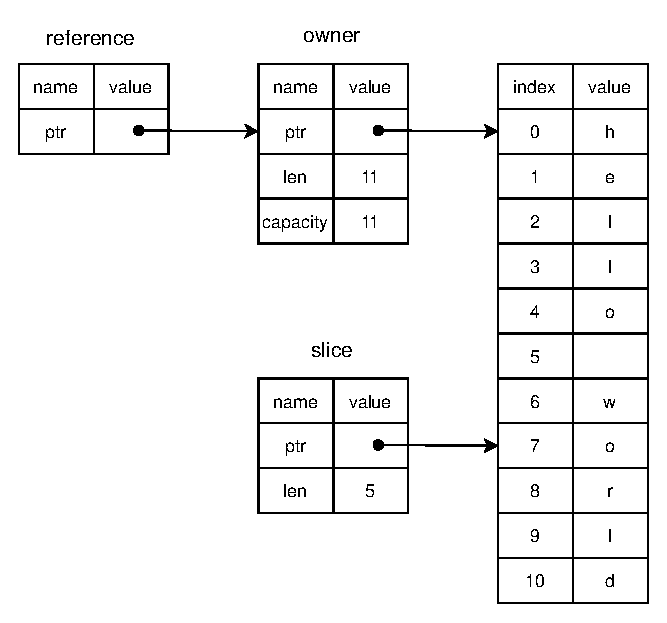
\includegraphics[width=0.5\textwidth]{images/own_ref_slice.eps}
                \captionsetup{labelformat=empty}
                % \caption{\textbf{}}
        \end{center}
    \end{figure}

    Each one may have \textcolor{blue}{different memory access time.}
\end{frame}

%%%%%%%%%%%%%%%%%%%%%%%%%%%%%%%%%%%%%%%%%%%%
%%%%%%%%%%%%%%%%%%%%%%%%%%%%%%%%%%%%%%%%%%%%

\begin{frame}[fragile]{Reference Counting}

    \textbf{Advantage}
    \begin{itemize}
        \item \blue{Sharing ownership} 
        \item \blue{Dinamic memory de/allocation}
    \end{itemize}

    \vspace{0.5cm}

    \textbf{Disadvantage}
    \begin{itemize}
        \item \blue{Need to check reference count} 
        \item \blue{Heap allocation}
    \end{itemize}


\end{frame}

%%%%%%%%%%%%%%%%%%%%%%%%%%%%%%%%%%%%%%%%%%%%
%%%%%%%%%%%%%%%%%%%%%%%%%%%%%%%%%%%%%%%%%%%%

\begin{frame}[fragile]{Multithreading with Atomic Reference Counting}
    Atomic Reference Counting

    \vspace{0.5cm}
    \textbf{Advantage}
    \begin{itemize}
        \item \blue{Sharing ownership} 
        \item \blue{Dinamic memory de/allocation}
        \item \blue{Sharing among multithreads}
    \end{itemize}

    \vspace{0.5cm}

    \textbf{Disadvantage}
    \begin{itemize}
        \item \blue{Need to check reference count} 
        \item \blue{Heap allocation}
        \item \blue{Atomic operation} 
    \end{itemize}

\end{frame}

%%%%%%%%%%%%%%%%%%%%%%%%%%%%%%%%%%%%%%%%%%%%
%%%%%%%%%%%%%%%%%%%%%%%%%%%%%%%%%%%%%%%%%%%%

\begin{frame}[fragile]{Impact of Memory Management on performance of Big Data Processing}

    \begin{itemize}
        \item \blueb{Merge-sort}
        \begin{itemize}
            \item Many contiguous memory de/allocations
        \end{itemize}
        \vspace{0.5cm}
        \item \blueb{Tree-aggtegate}
        \begin{itemize}
            \item Many intermediate HashMap like data structures
        \end{itemize}
        \vspace{0.5cm}
        \item \blueb{K-Nearest-Neighbors (KNN)}
        \begin{itemize}
            \item Document preprocessing 
        \end{itemize}    
    \end{itemize}

\end{frame}

%%%%%%%%%%%%%%%%%%%%%%%%%%%%%%%%%%%%%%%%%%%%
%%%%%%%%%%%%%%%%%%%%%%%%%%%%%%%%%%%%%%%%%%%%

\begin{frame}[fragile]{Experiment 1: Accessing Object with Different Variable Type}

    \textbf{Question}
    \begin{itemize}
        \item How much are memory access times different among different memory management strategies used in complex objects?
    \end{itemize}

    \vspace{0.5cm}

    \textbf{Evaluation}
    \begin{itemize}
        \item \blueb{Custruct complext objects}
        \item With different memory management strategies: \blueb{Owner, Reference, Slice}
        \item CustomerOwned vs. CustomerBorrowed vs. CustomerSlice
        \item Measure time to \blueb{access to fields of complex objects}
    \end{itemize}

\end{frame}

%%%%%%%%%%%%%%%%%%%%%%%%%%%%%%%%%%%%%%%%%%%%
%%%%%%%%%%%%%%%%%%%%%%%%%%%%%%%%%%%%%%%%%%%%

\begin{frame}[t, fragile]{Experiment 1: Accessing Object with Different Variable Type}

    \begin{figure}[hp]
        \centering
        \begin{center}
                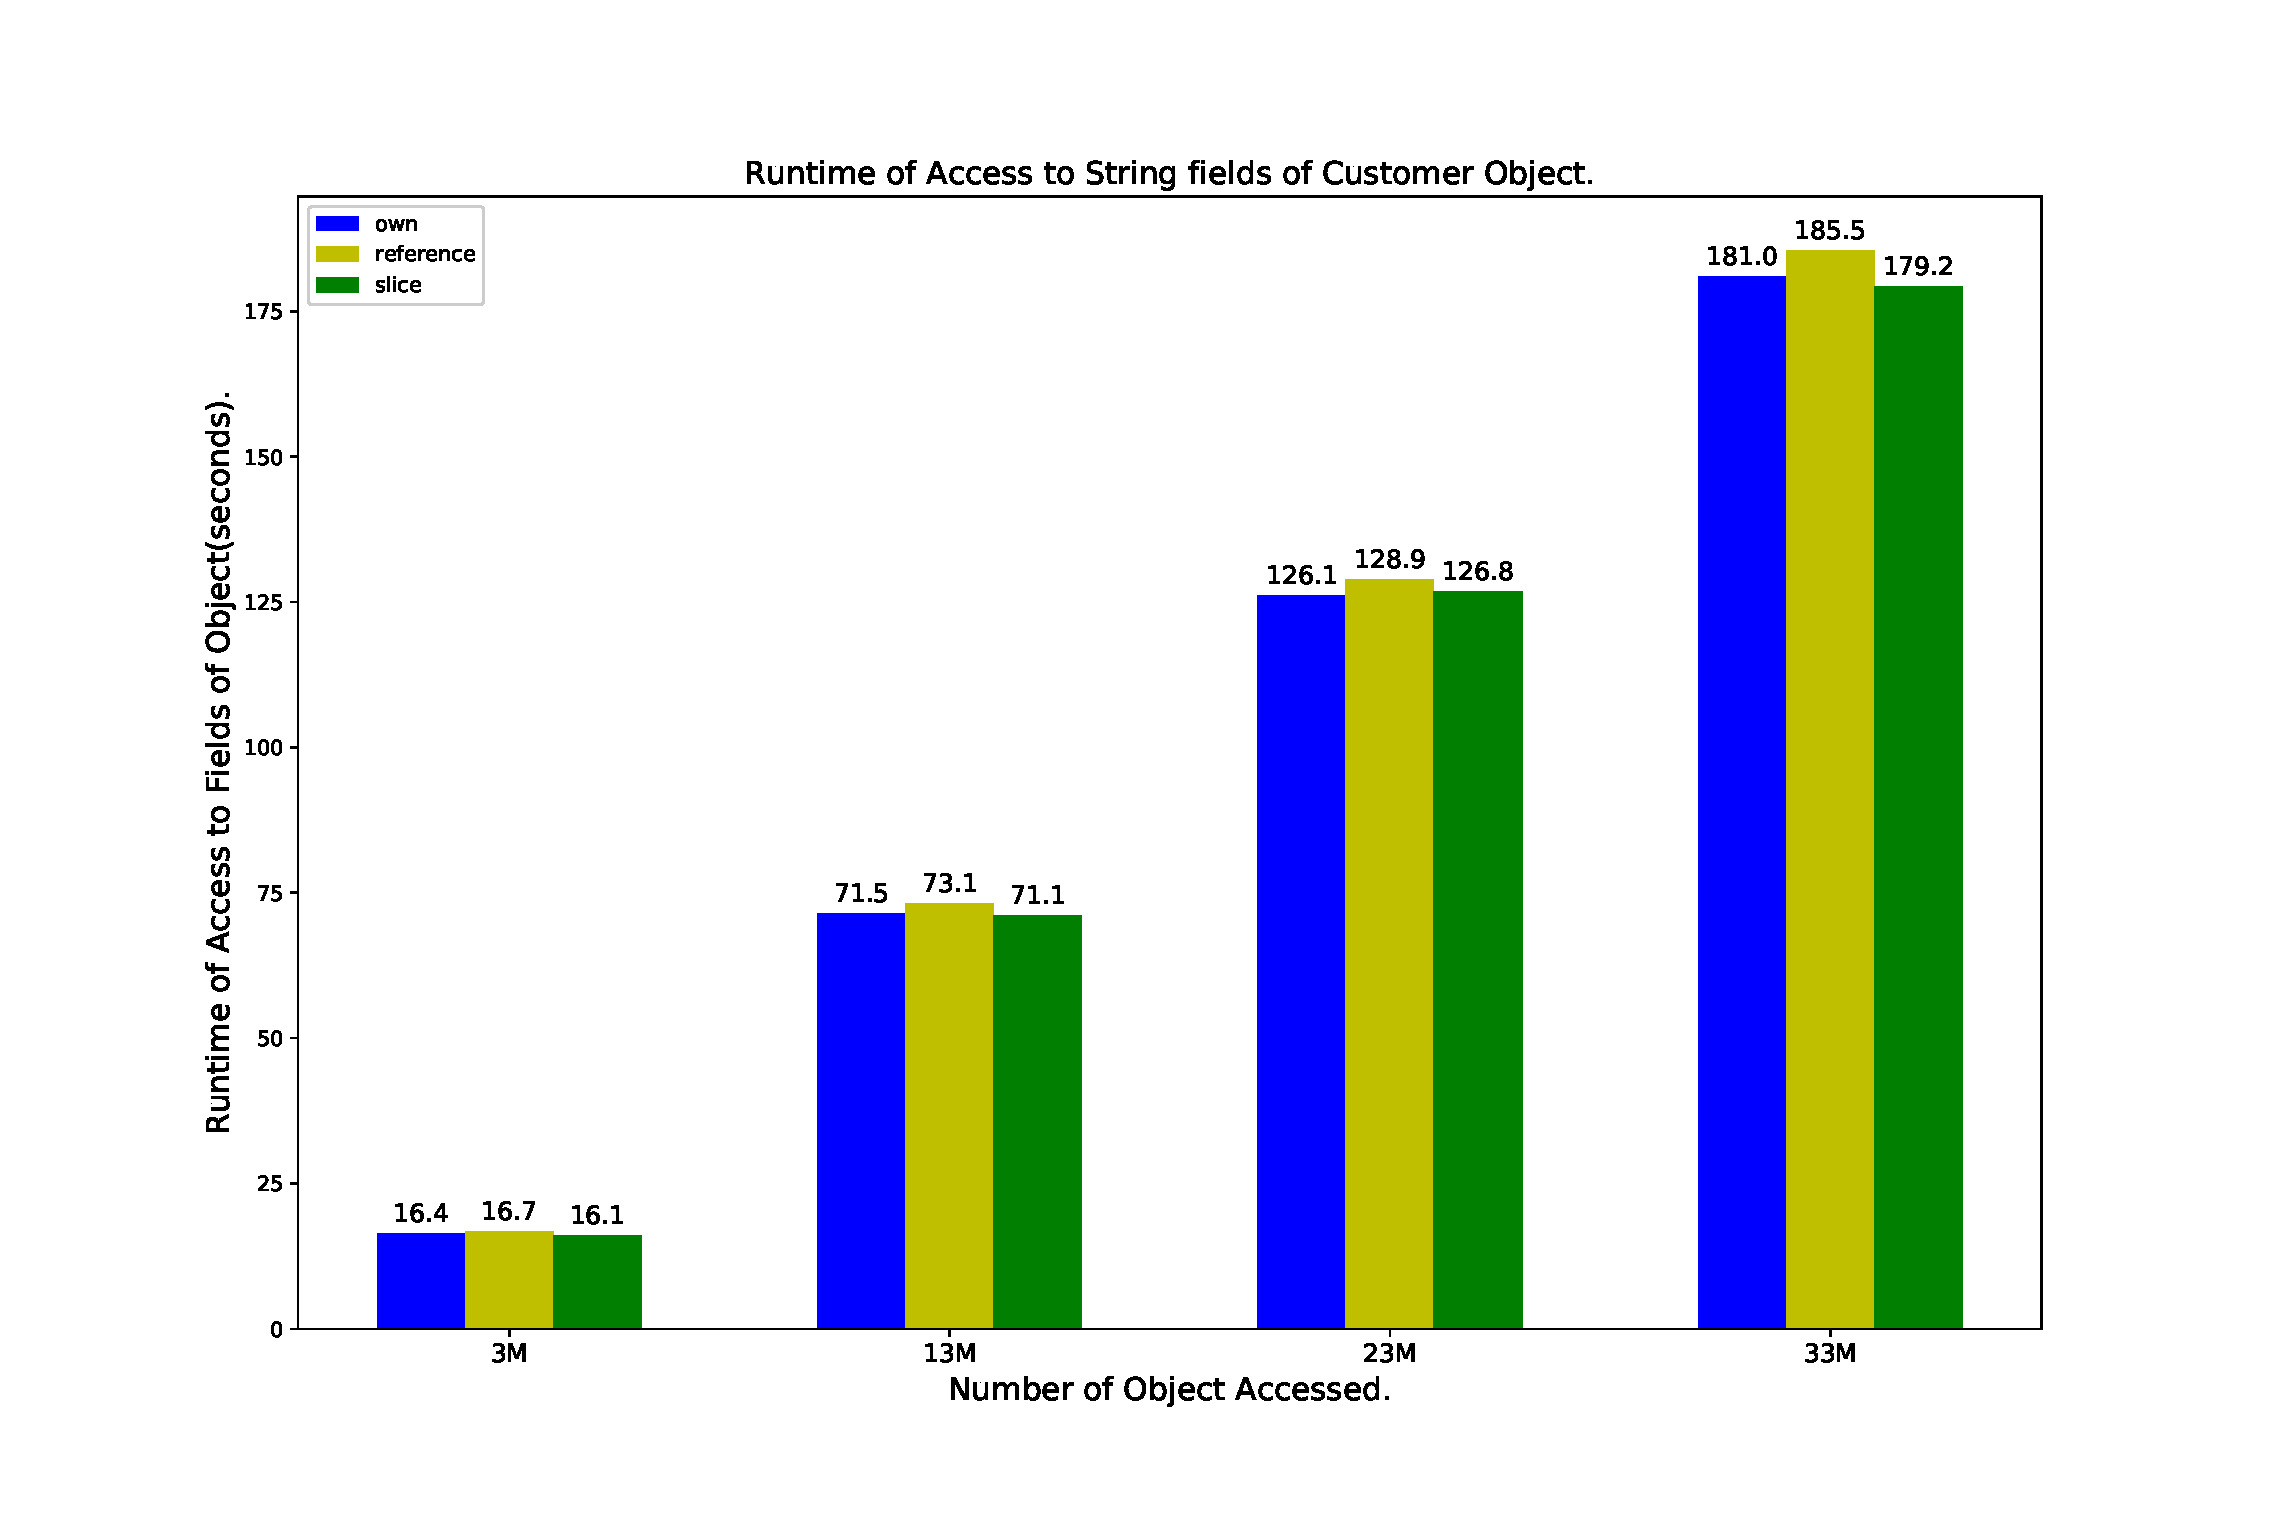
\includegraphics[width=1\textwidth]{images/rust_access_different_poniter_init.eps}
                \captionsetup{labelformat=empty}
                % \caption{\textbf{}}
        \end{center}
    \end{figure}
\end{frame}

%%%%%%%%%%%%%%%%%%%%%%%%%%%%%%%%%%%%%%%%%%%%
%%%%%%%%%%%%%%%%%%%%%%%%%%%%%%%%%%%%%%%%%%%%

\begin{frame}[fragile]{Experiment 2: Assessment of different reference methods in Rust}

    \textbf{Question}
    \begin{itemize}
        \item How much does Reference Counting slowdown time for dropping its variable?
    \end{itemize}

    \vspace{0.5cm}

    \textbf{Evaluation}
    \begin{itemize}
        \item \blueb{Custruct complext objects}
        \item \blueb{Reference Counting} vs \blueb{reference}
        \item CustomerRc vs. CustomerBorrowed
        \item Measure time to \blueb{drop variables of complex objects}
    \end{itemize}

\end{frame}

%%%%%%%%%%%%%%%%%%%%%%%%%%%%%%%%%%%%%%%%%%%%
%%%%%%%%%%%%%%%%%%%%%%%%%%%%%%%%%%%%%%%%%%%%


\begin{frame}[fragile]{Experiment 2: Assessment of different reference methods in Rust}

    \begin{figure}[hp]
        \centering
        \begin{center}
                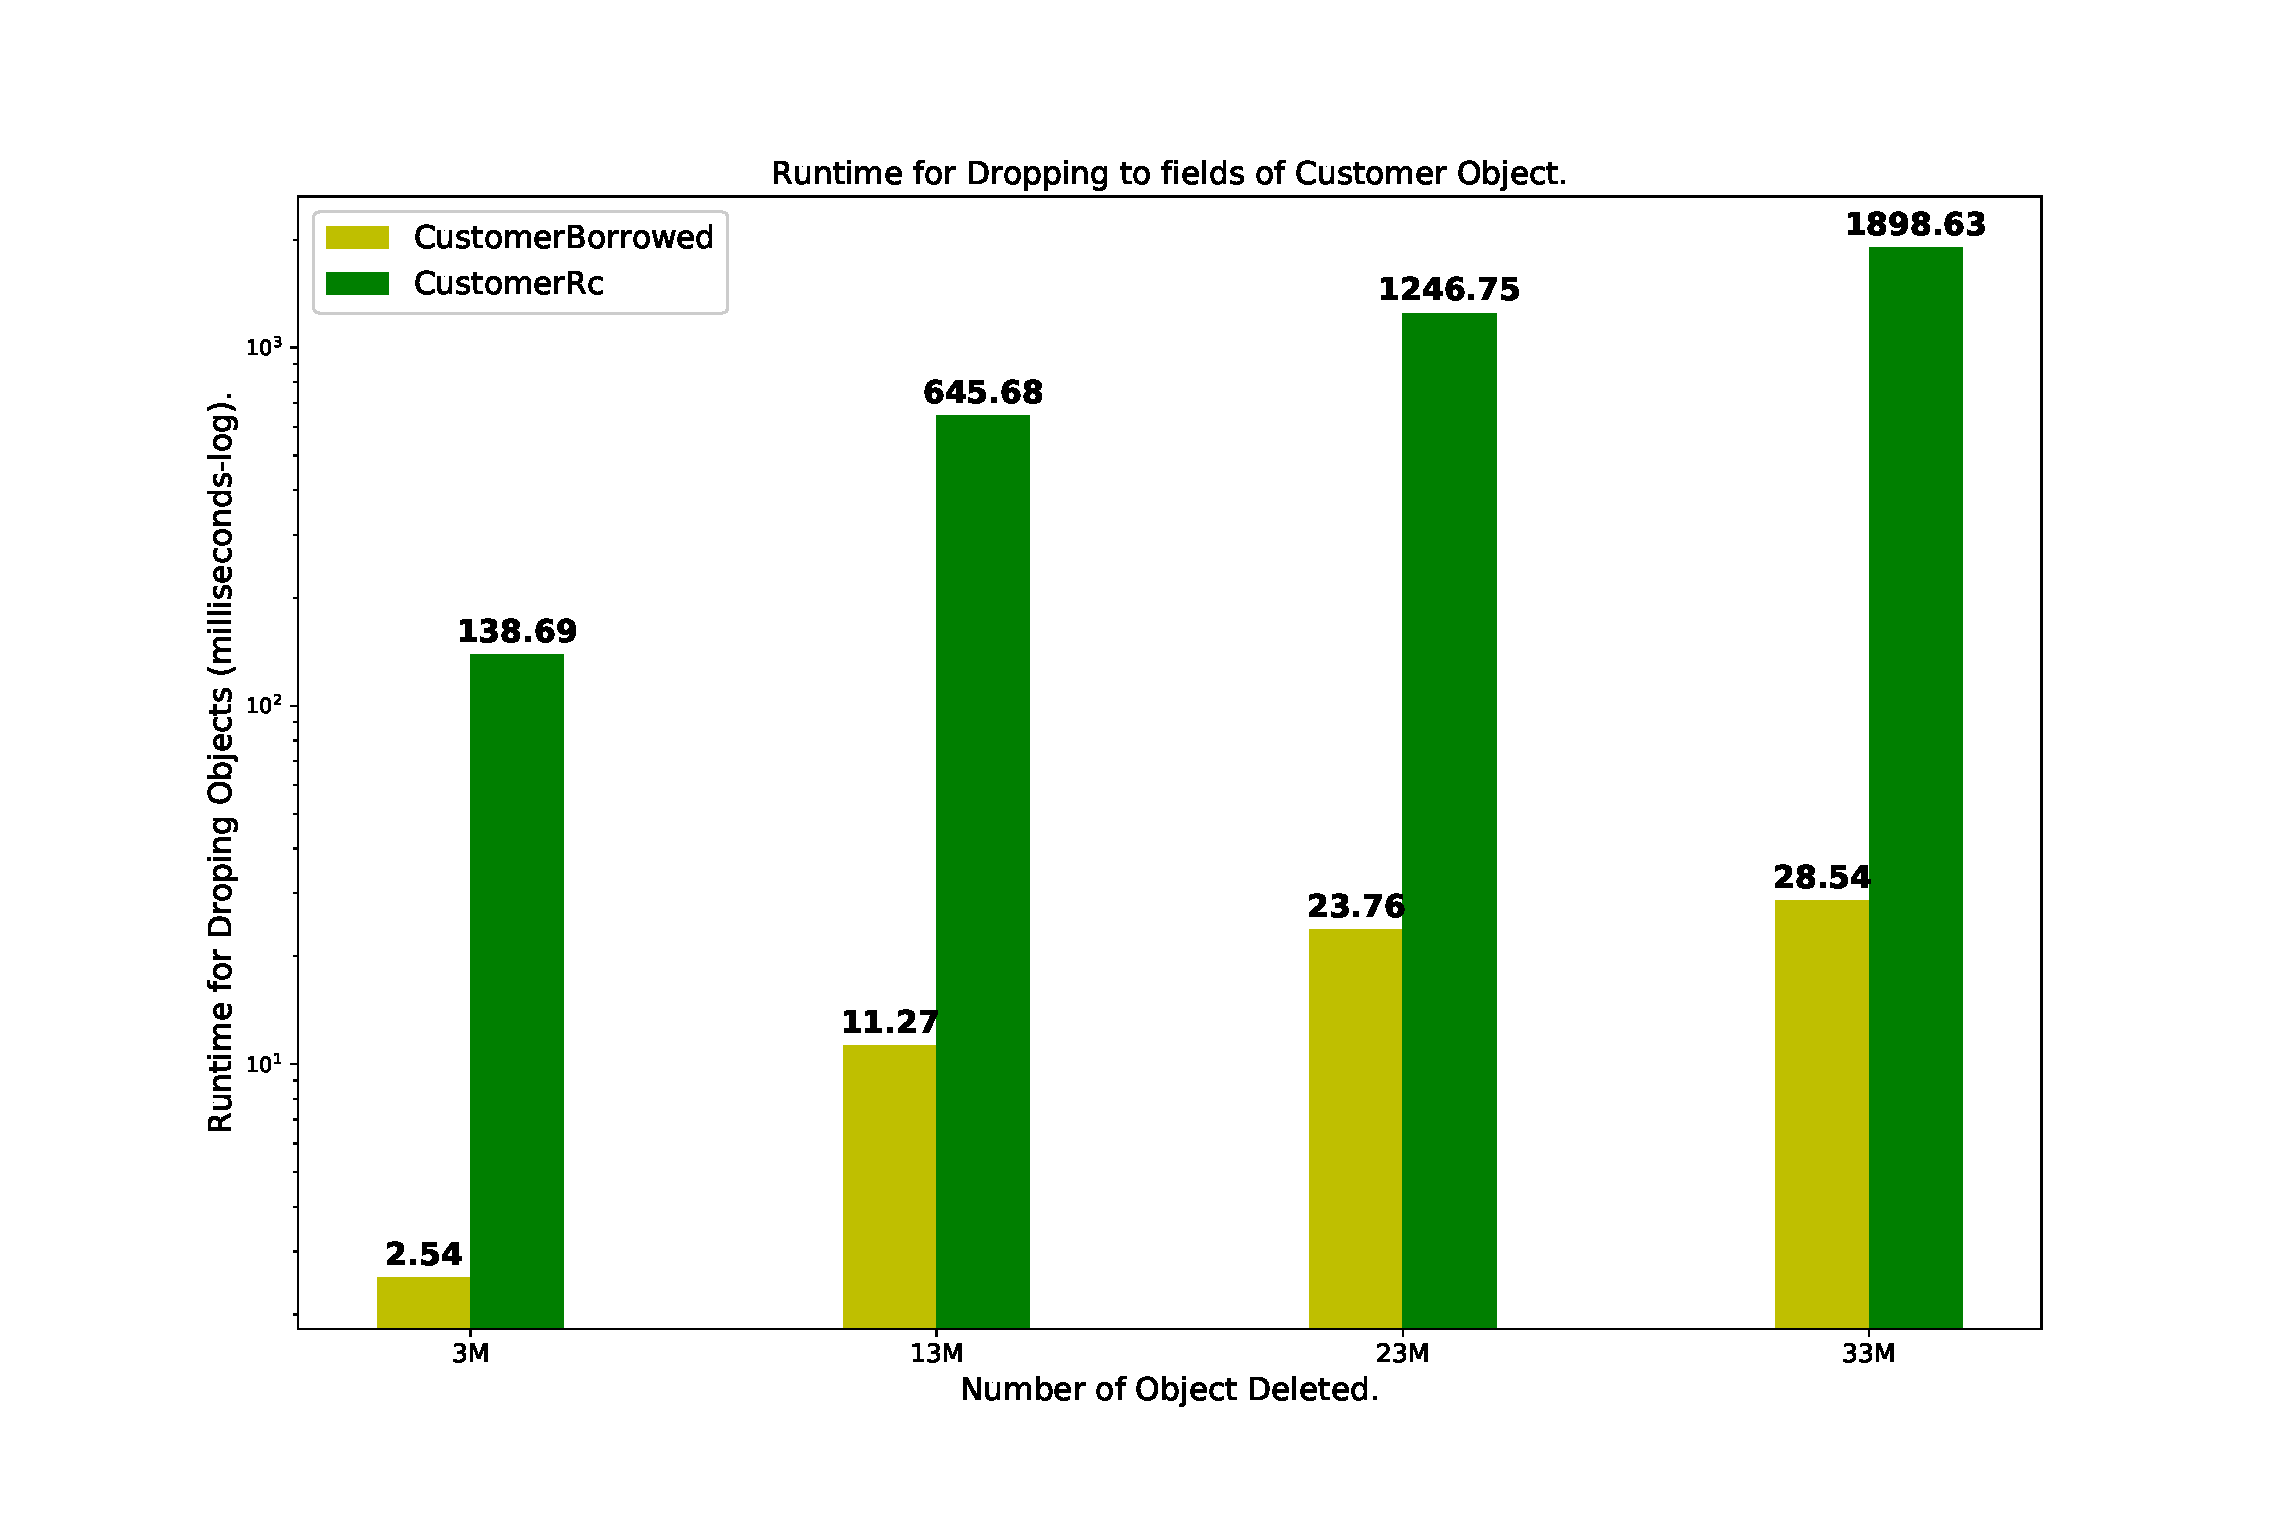
\includegraphics[width=1\textwidth]{images/rust_droptime_borring_rc.eps}
                \captionsetup{labelformat=empty}
                % \caption{\textbf{}}
        \end{center}
    \end{figure}
\end{frame}
%%%%%%%%%%%%%%%%%%%%%%%%%%%%%%%%%%%%%%%%%%%%
%%%%%%%%%%%%%%%%%%%%%%%%%%%%%%%%%%%%%%%%%%%%

\begin{frame}[fragile]{Experiment 2: Assessment of different reference methods in Rust}
    \textbf{Result}
    \begin{itemize}
        \item Dropping Reference Counting is about \blueb{60 times slower} than normal reference.
    \end{itemize}

    \vspace{0.5cm}

    \textbf{Discussion}
    \begin{itemize}
        \item Reference Counting needs to check reference count.
        \item In complex objects, overhead is significant.
    \end{itemize}
\end{frame}

%%%%%%%%%%%%%%%%%%%%%%%%%%%%%%%%%%%%%%%%%%%%
%%%%%%%%%%%%%%%%%%%%%%%%%%%%%%%%%%%%%%%%%%%%

\begin{frame}[fragile]{Experiment 3: Merge-sort}

    \textbf{Question}
    \begin{itemize}
        \item How much does sharing set of data with Atomic Reference Counting slowdown merge-sort algorithms?
    \end{itemize}

    \vspace{0.5cm}

    \textbf{Evaluation}
    \begin{itemize}
        \item Share \blueb{vector} of complex objects
        \item \blueb{Atomic Reference Counting (Arc)} vs \blueb{normal reference}
        \item Measure \blueb{runtime of merge-sort algorithms}
    \end{itemize}

\end{frame}

%%%%%%%%%%%%%%%%%%%%%%%%%%%%%%%%%%%%%%%%%%%%
%%%%%%%%%%%%%%%%%%%%%%%%%%%%%%%%%%%%%%%%%%%%


\begin{frame}[fragile]{Experiment 3: Merge-sort}
    \vspace{-0.7cm}
    \begin{figure}[hp]
        \centering
        \begin{center}
                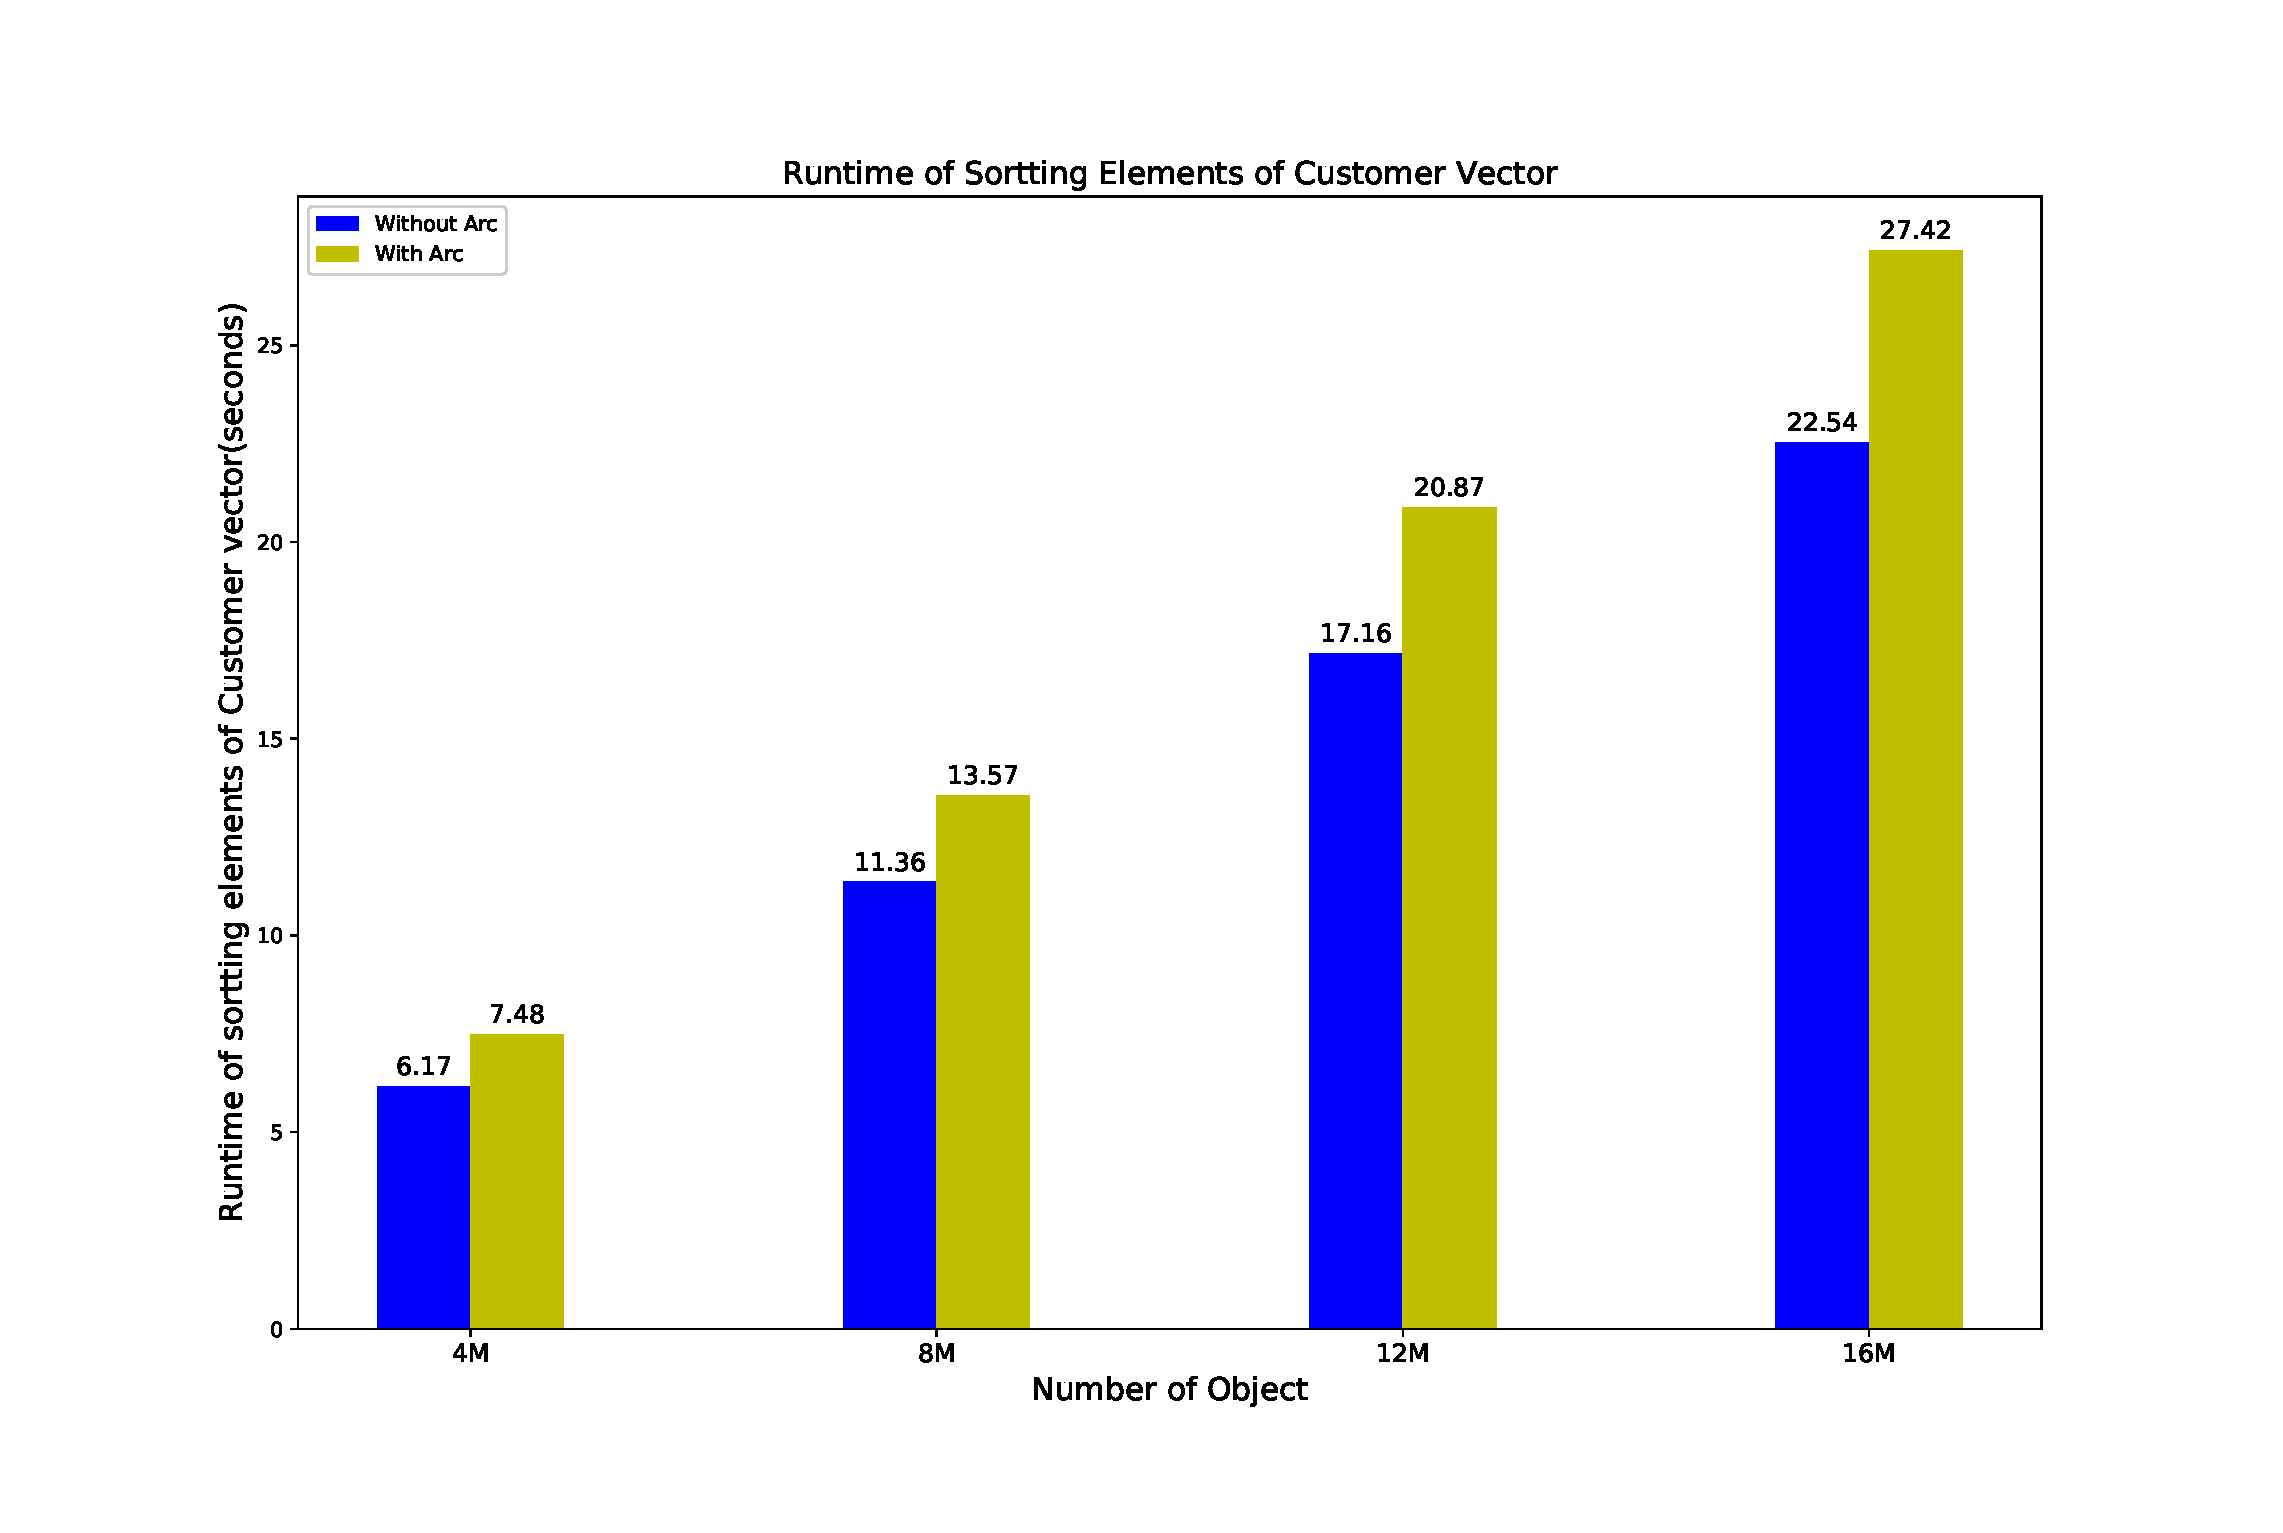
\includegraphics[width=1.1\textwidth]{images/rust_merge_sort.eps}
                \captionsetup{labelformat=empty}
                % \caption{\textbf{}}
        \end{center}
    \end{figure}
\end{frame}

%%%%%%%%%%%%%%%%%%%%%%%%%%%%%%%%%%%%%%%%%%%%
%%%%%%%%%%%%%%%%%%%%%%%%%%%%%%%%%%%%%%%%%%%%

\begin{frame}[fragile]{Experiment 3: Merge-sort}

    \textbf{Result}
    \begin{itemize}
        \item Arc are about \blueb{21\%  slower} than normal reference.
    \end{itemize}

    \vspace{0.5cm}

    \textbf{Discussion}
    \begin{itemize}
        \item Atomic Reference Counting needs to check reference count.
        \item Atomic operations are more expensive than ordinal operations.
    \end{itemize}

\end{frame}

%%%%%%%%%%%%%%%%%%%%%%%%%%%%%%%%%%%%%%%%%%%%
%%%%%%%%%%%%%%%%%%%%%%%%%%%%%%%%%%%%%%%%%%%%

\begin{frame}[fragile]{Experiment 4: Tree-aggregate}

    \textbf{Question}
    \begin{itemize}
        \item How much are runtime differences between sharing elements of data with Arc and deep-copying elements of data?
    \end{itemize}

    \vspace{0.5cm}

    \textbf{Evaluation}
    \begin{itemize}
        \item Share \blueb{elements} of complex object
        \item \blueb{Atomic Reference Counting (ARC)} vs \blueb{Deep copy}
        \item Measure \blueb{runtime of Tree-aggregate algorithms}
    \end{itemize}

\end{frame}

%%%%%%%%%%%%%%%%%%%%%%%%%%%%%%%%%%%%%%%%%%%%
%%%%%%%%%%%%%%%%%%%%%%%%%%%%%%%%%%%%%%%%%%%%

\begin{frame}[t, fragile]{Experiment 4: Tree-aggregate}
    \vspace{-0.7cm}
    \begin{figure}[hp]
        \centering
        \begin{center}
                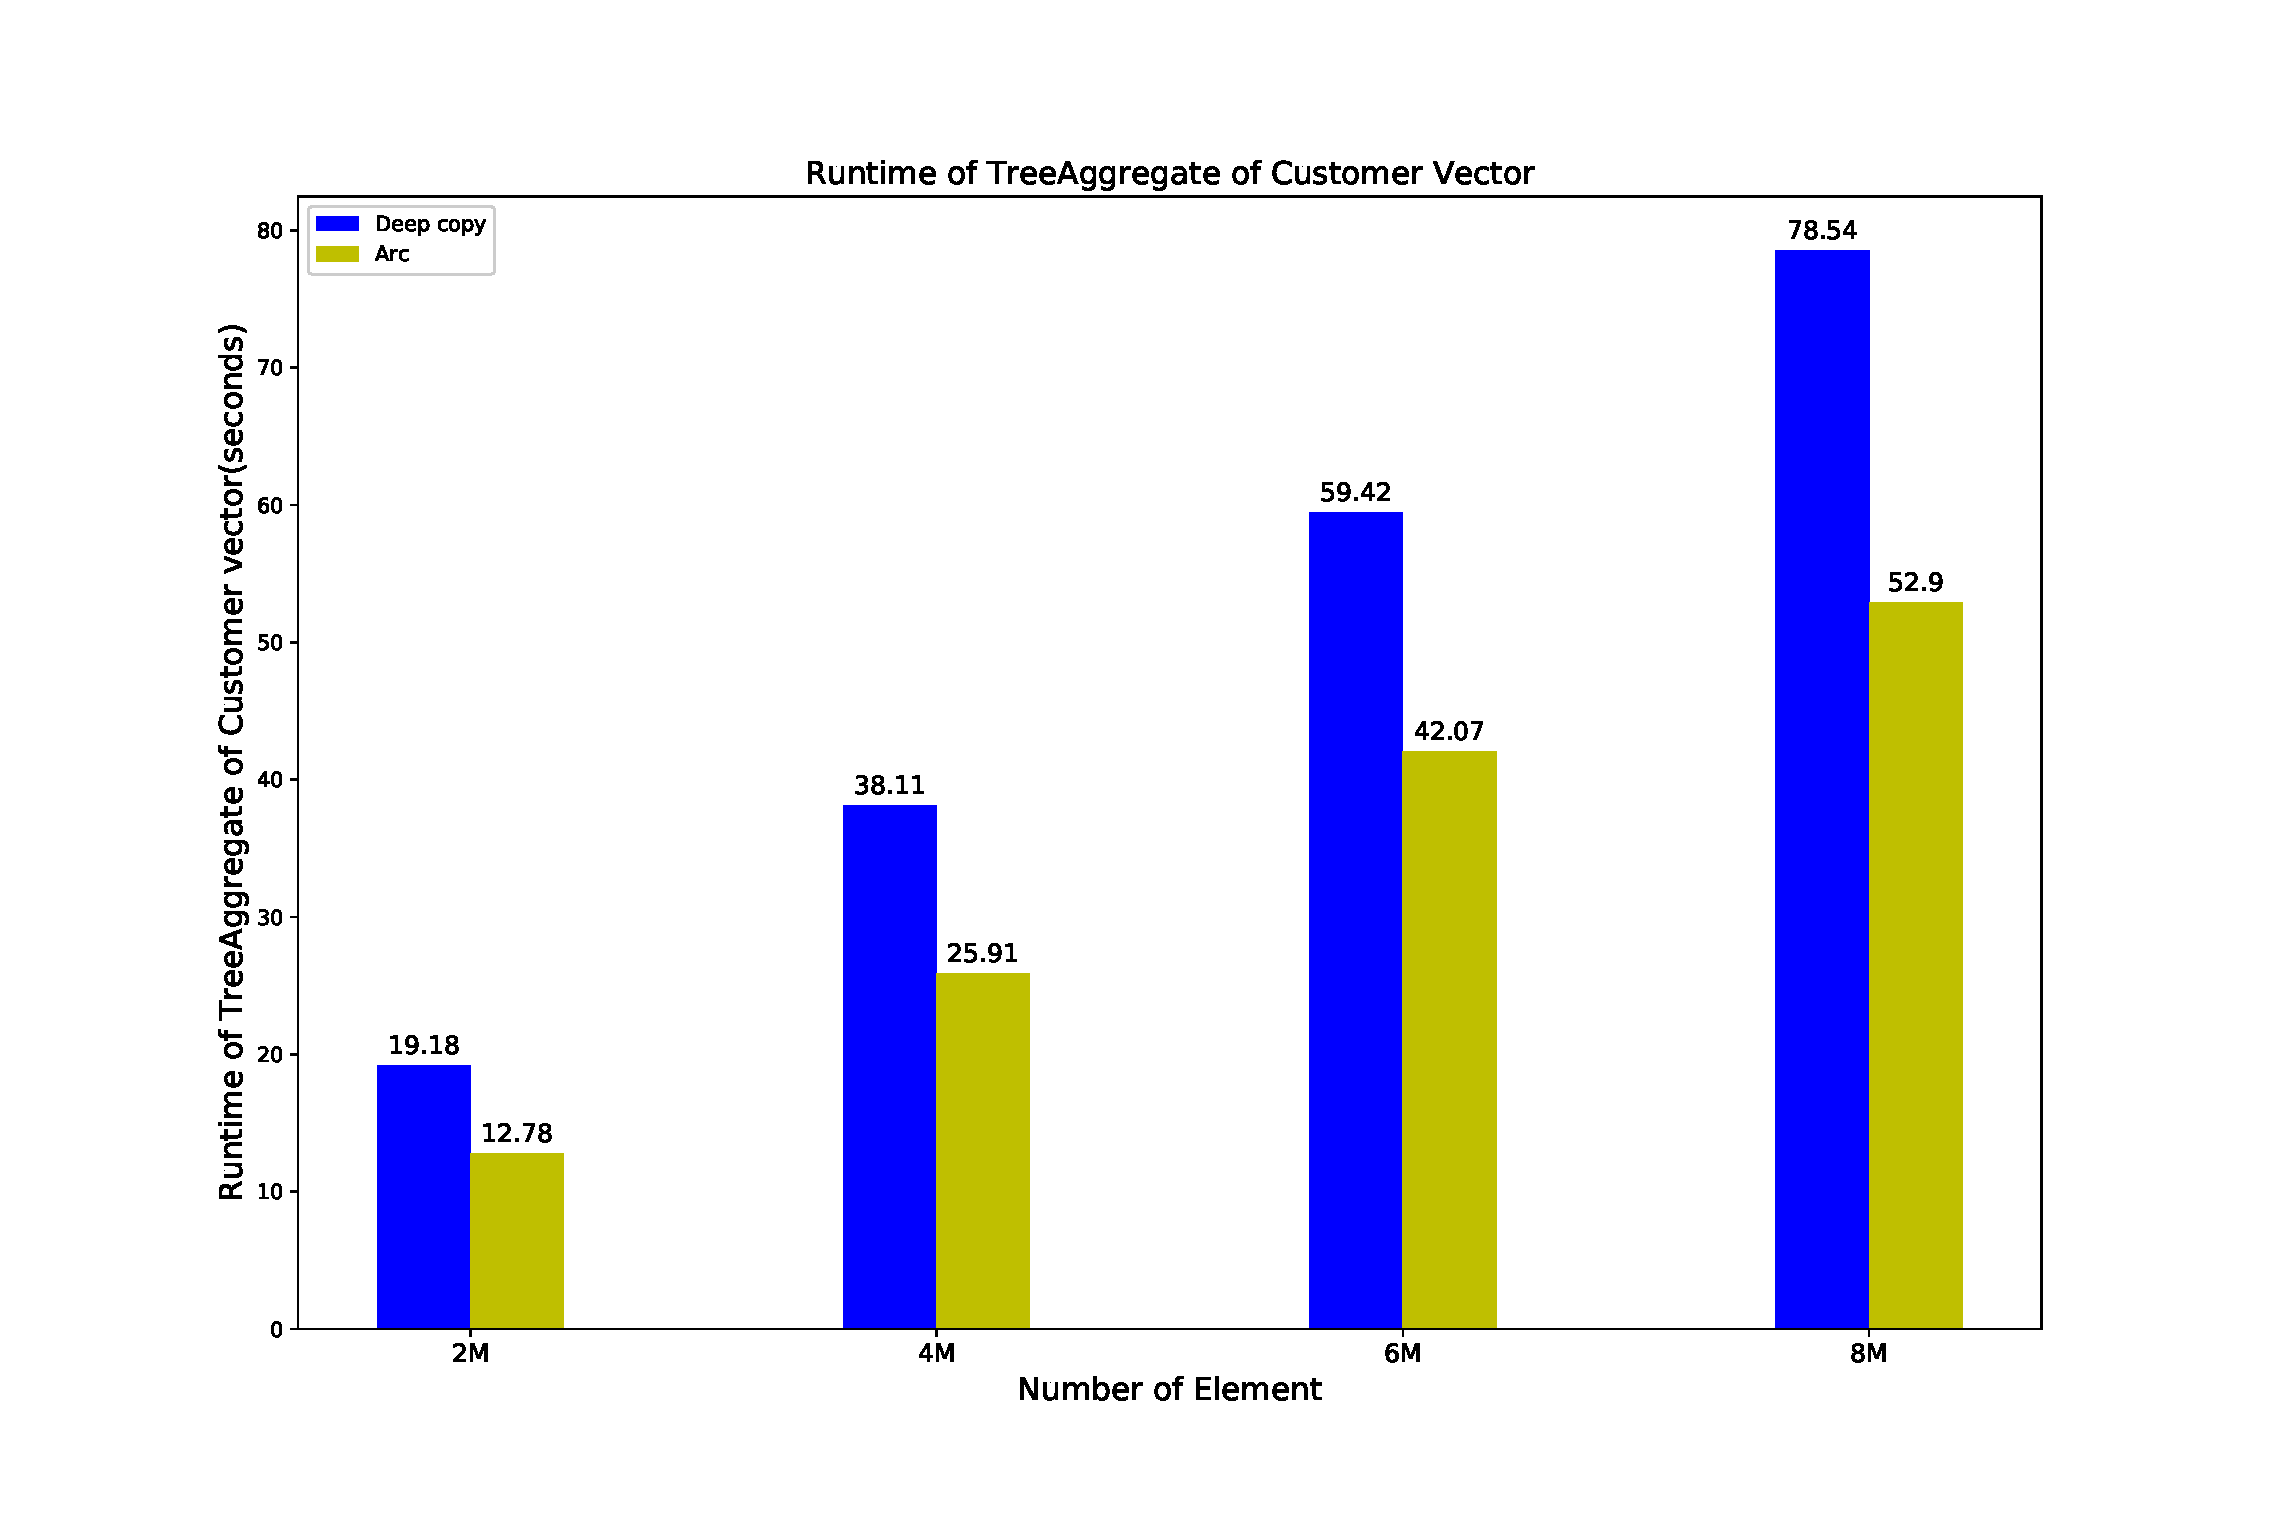
\includegraphics[width=1.1\textwidth]{images/rust_tree_aggregate.eps}
                \captionsetup{labelformat=empty}
                % \caption{\textbf{}}
        \end{center}
    \end{figure}
\end{frame}

%%%%%%%%%%%%%%%%%%%%%%%%%%%%%%%%%%%%%%%%%%%%
%%%%%%%%%%%%%%%%%%%%%%%%%%%%%%%%%%%%%%%%%%%%

\begin{frame}[fragile]{Experiment 4: Tree-aggregate}

    \textbf{Result}
    \begin{itemize}
        \item Deep-copies are from \blueb{40 to 50\% slower} than Arc.
    \end{itemize}

    \vspace{0.5cm}

    \textbf{Discussion}
    \begin{itemize}
        \item Deep-copy of complex object is expensive.
        \item Performing deep-copy many times may lead significant overhead.
    \end{itemize}

\end{frame}

%%%%%%%%%%%%%%%%%%%%%%%%%%%%%%%%%%%%%%%%%%%%
%%%%%%%%%%%%%%%%%%%%%%%%%%%%%%%%%%%%%%%%%%%%
\begin{frame}[fragile]{Experiment 5: K-Nearest-Neighbors (KNN)}

    \textbf{Question}
    \begin{itemize}
        \item What are better memory management strategies for common Machine Learning Algorithms?
    \end{itemize}

    \vspace{0.5cm}

    \textbf{Evaluation}
    \begin{itemize}
        \item Document classification on Wikipedia page dataset
        \begin{itemize}
            \item train set: \(100 \times 10^3 \) pages
            \item test set: \(18 \times  10^3\) pages
        \end{itemize}
        \item Preprocessing phase: calculating \blueb{Term-Frequencies (TFs)}
        \item String manipulation
        \item Measure runtime of \blueb{preprocessing time of KNN algorithms}
    \end{itemize}
\end{frame}

%%%%%%%%%%%%%%%%%%%%%%%%%%%%%%%%%%%%%%%%%%%%
%%%%%%%%%%%%%%%%%%%%%%%%%%%%%%%%%%%%%%%%%%%%

\begin{frame}[fragile]{Experiment 5: K-Nearest-Neighbors (KNN)}

    \blueb{Parameters}
    \begin{itemize}
        \item Data Acquisition
        \begin{itemize}
            \item \blueb{Atomic Reference Counting} (Arc)
            \item \blueb{Deep-copy}
        \end{itemize} 
        \vspace{0.5cm}
        \item Strategy
        \begin{itemize}
            \item keep intermediate objects in memory until owner is changed
            \item remove intermediate objects as soon as it is not needed
        \end{itemize}
        \vspace{0.5cm}
        \item Dimensions of feature matrices
        \begin{itemize}
            \item 15K
            \item 20K
            \item 25K
        \end{itemize} 
    \end{itemize}
\end{frame}

%%%%%%%%%%%%%%%%%%%%%%%%%%%%%%%%%%%%%%%%%%%%
%%%%%%%%%%%%%%%%%%%%%%%%%%%%%%%%%%%%%%%%%%%%

\begin{frame}[fragile]{Experiment 5: K-Nearest-Neighbors}
    \vspace{-0.7cm}
    \begin{figure}[hp]
        \centering
        \begin{center}
                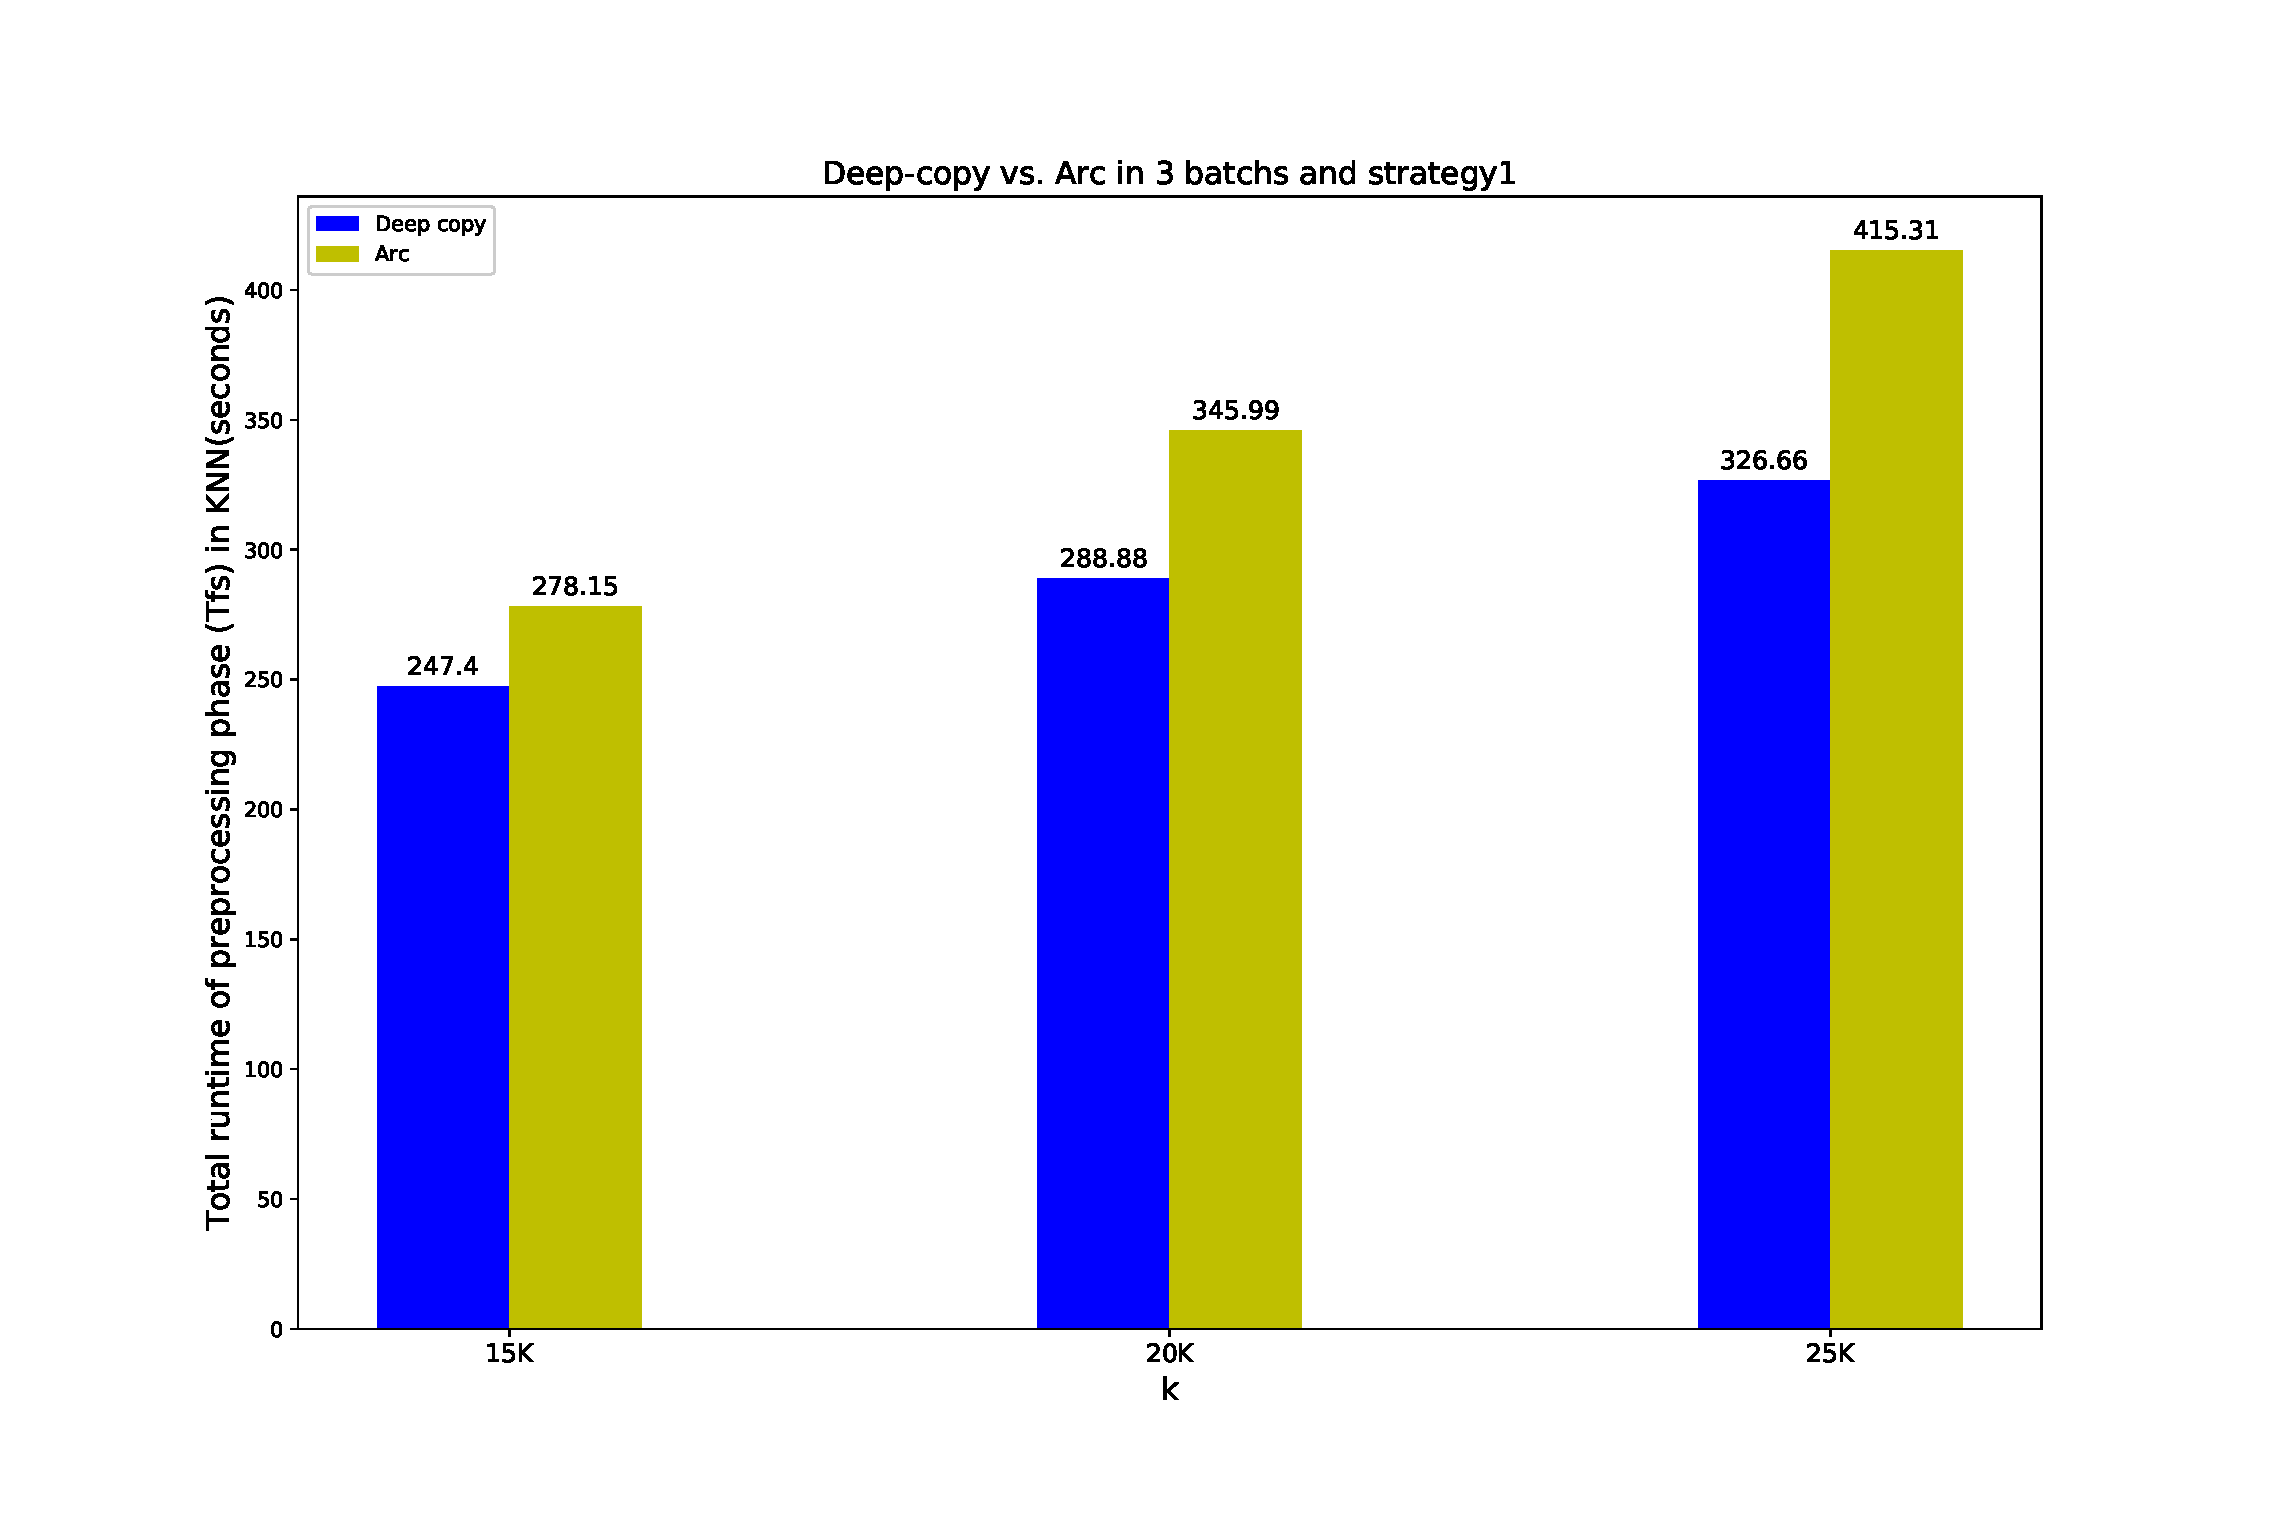
\includegraphics[width=1.1\textwidth]{images/deepcopy_vs_arc.eps}
                \captionsetup{labelformat=empty}
                % \caption{\textbf{}}
        \end{center}
    \end{figure}
    
\end{frame}

%%%%%%%%%%%%%%%%%%%%%%%%%%%%%%%%%%%%%%%%%%%%
%%%%%%%%%%%%%%%%%%%%%%%%%%%%%%%%%%%%%%%%%%%%

\begin{frame}[fragile]{Experiment 5: K-Nearest-Neighbors}
    \vspace{-0.7cm}
    \begin{figure}[hp]
        \centering
        \begin{center}
                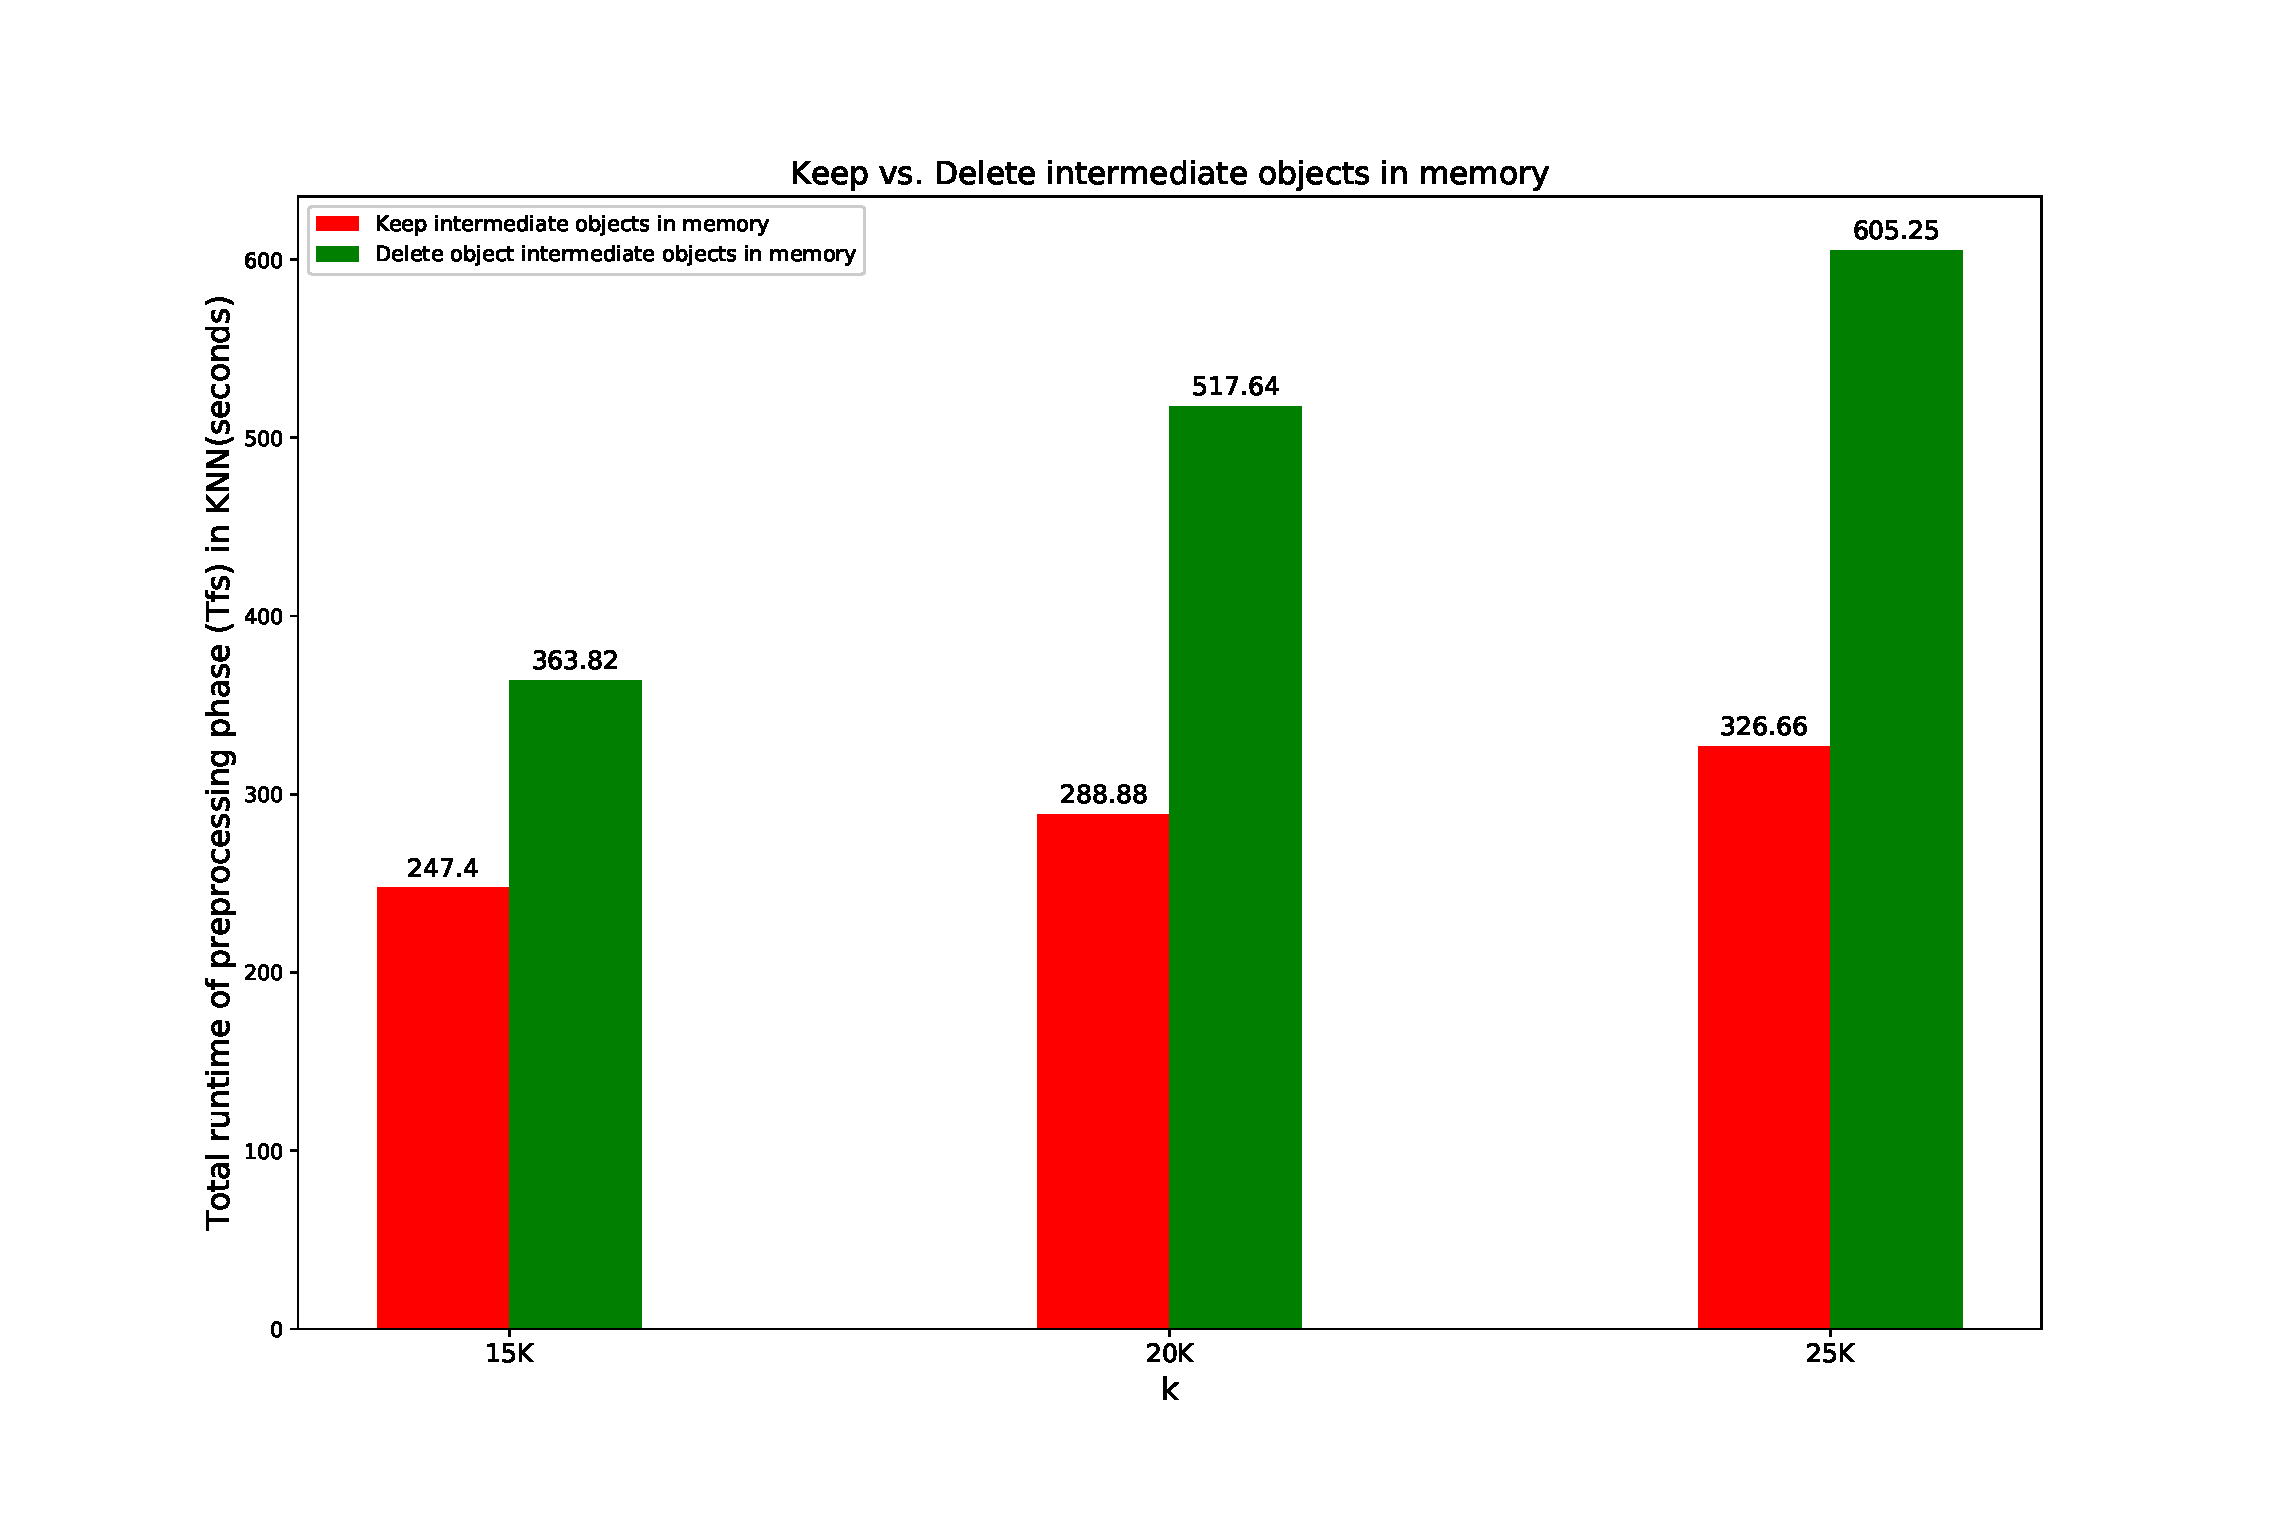
\includegraphics[width=1.1\textwidth]{images/strategy1_vs_strategy2.eps}
                \captionsetup{labelformat=empty}
                % \caption{\textbf{}}
        \end{center}
    \end{figure}
    
\end{frame}

%%%%%%%%%%%%%%%%%%%%%%%%%%%%%%%%%%%%%%%%%%%%
%%%%%%%%%%%%%%%%%%%%%%%%%%%%%%%%%%%%%%%%%%%%


\begin{frame}[fragile]{Experiment 5: K-Nearest-Neighbors}
    
    \textbf{Result}
    \begin{itemize}
        \item \blueb{Arc} is \blueb{at most 38\% slower} than deep-copy.
        \item Removing intermediate objects is \blueb{at most 85\% slower} than keeping the objects.
    \end{itemize}

    \vspace{0.5cm}

    \textbf{Discussion}
    \begin{itemize}
        \item Deep-copying String is cheaper operation than Arc: 
        \begin{itemize}
            \item reference checking
            \item atomic operation
        \end{itemize}
        \item More frequent deallocation of intermediate objects may lead to overhead.
    \end{itemize} 
\end{frame}

%%%%%%%%%%%%%%%%%%%%%%%%%%%%%%%%%%%%%%%%%%%%
%%%%%%%%%%%%%%%%%%%%%%%%%%%%%%%%%%%%%%%%%%%%

\begin{frame}[fragile]{Conclusion}
    \begin{itemize}
        \item There are \blue{not notable differences} among times to access memory with different memory management strategies.
        \item When we drop complex objects constructed with Reference Counting, \blue{additional computation for counting reference results in huge overhead}. 
        \item \blue{Sharing set of data with Arc is more expensive than reference.}
        \item \blue{Deep-copying complex objects is more expensive than sharing them with Arc.}
        \item \blue{Sharing Strings with Arc is faster than deep-copying them.}
    \end{itemize}
\end{frame}


%%%%%%%%%%%%%%%%%%%%%%%%%%%%%%%%%%%%%%%%%%%%
%%%%%%%%%%%%%%%%%%%%%%%%%%%%%%%%%%%%%%%%%%%%

\begin{frame}[fragile]{Findings}
    \begin{itemize}
        \item Use normal reference rather than Reference Counting whenever it is possible.
        \item Trade-off between \blueb{runtime performance} and \blueb{lifetime tracking}.
        \item \blueb{Avoid using Arc} when we can use reference.
        \item Use Arc instead of deep-copy, when \blueb{complexity of objects is large}.
        \item Use deep-copy, when \blueb{complexity of objects is small}, like String.
    \end{itemize}
\end{frame}


% \section{Some Terminology}

% \begin{frame}[fragile, t ]{Convex Function}
% A function $f(x)$ is defined to be convex when
% \begin{align*}
% \forall x_1, x_2 \in X, \forall t \in [0,1]: f(t x_1 + (1 - t) x_2) \leq t f(x_1) + (1 - t) f(x_2)
% \end{align*}
% \vspace{-.5cm}

% \begin{minipage}{.49\linewidth}
% \begin{figure}[hp]
% \centering
% \begin{center}
%     	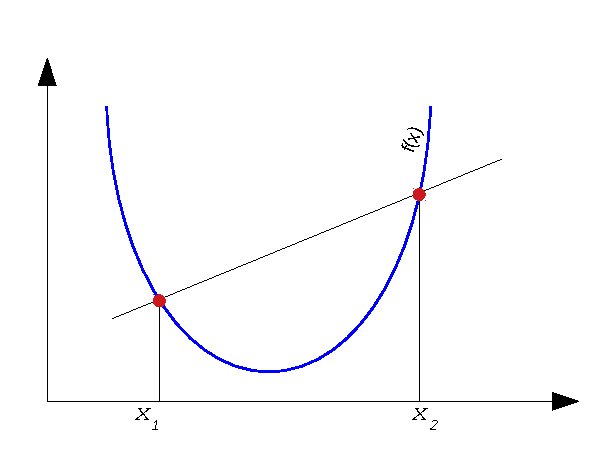
\includegraphics[width=1\textwidth]{images/convexFunction.pdf}
%     	\captionsetup{labelformat=empty}
%     	\caption{\textbf{Convex Function}}
% \end{center}
% \end{figure}
% \end{minipage}
% \pause
% \begin{minipage}{.49\linewidth}
% \begin{figure}[hp]
% \centering
% \begin{center}
%     	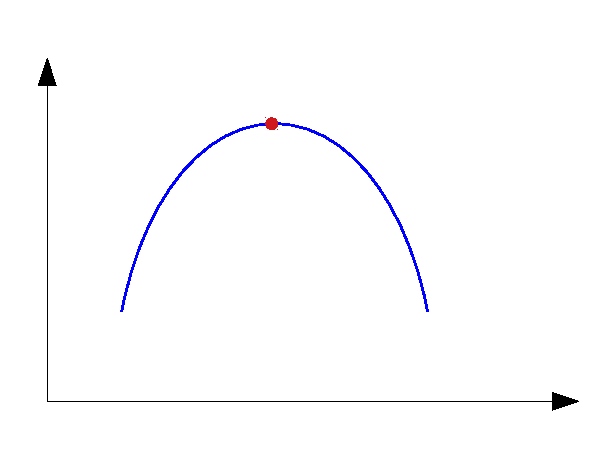
\includegraphics[width=1\textwidth]{images/concaveFunction.pdf}
%     	\captionsetup{labelformat=empty}
%     	\caption{\textbf{Concave Function}}
% \end{center}
% \end{figure}
% \end{minipage}
% \begin{itemize}
%   \item For maximum of a Concave function, we calculate minimum of $-f(x)$
% \end{itemize}

% \end{frame}


% %%%%%%%%%%%%%%%%%%%%%%%%%%%%%%%%%%%%%%%%%%%%
% %%%%%%%%%%%%%%%%%%%%%%%%%%%%%%%%%%%%%%%%%%%%

% \begin{frame}{None Convex Functions - Global and }

% \begin{center}
%     	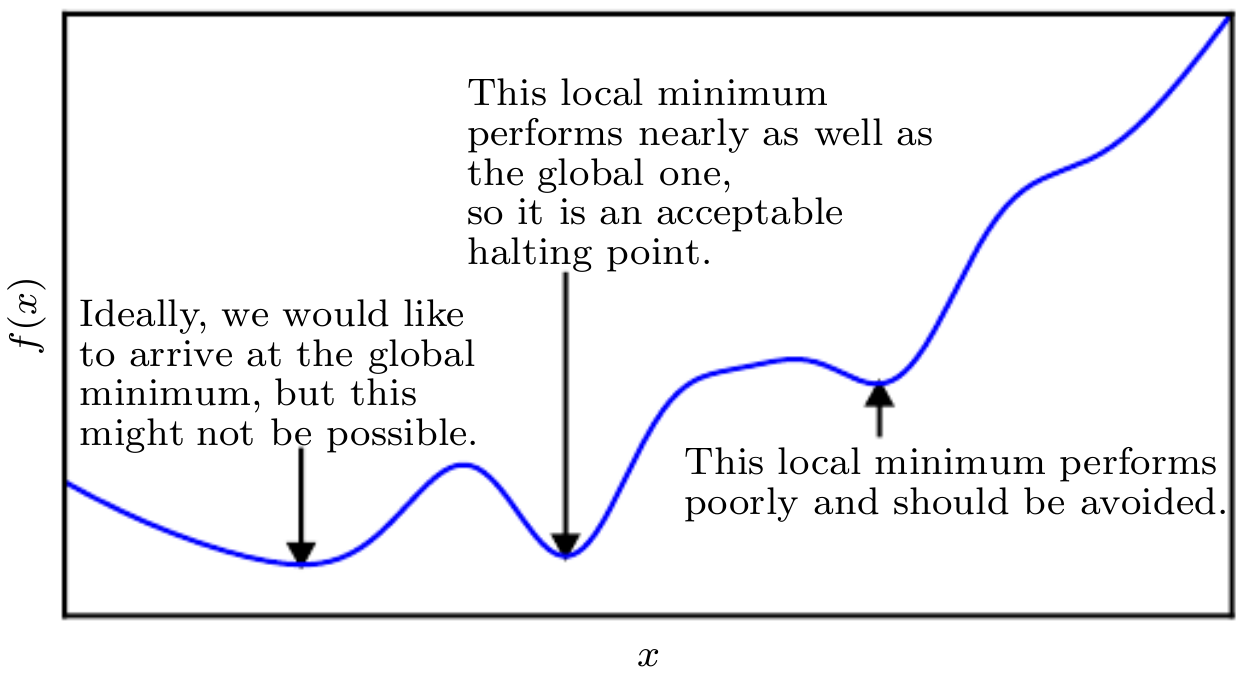
\includegraphics[width=0.8\textwidth]{images/GlobalMin.png}
% \scalebox{.5}{Image from Book:   Ian Goodfellow, Yoshua Bengio, Aaron Courville - Deep Learning - The MIT Press (2016)}

% \end{center}

% \end{frame}




% %
% %%%%%%%%%%%%%%%%%%%%%%%%%%%%%%%%%%%%%%%%%%%%%
% %%%%%%%%%%%%%%%%%%%%%%%%%%%%%%%%%%%%%%%%%%%%%
% %\section{Example - Doing Regression \\ Computation can be expensive}
% %\begin{frame}[fragile, t ]{Example - Doing Regression}
% %We have a set of training data like \\
% %
% %\begin{itemize}
% %\item Data Matrix of  \blueb{$X \in  \mathbb{R}^{n \times d}$},  with Labels \blueb{$Y \in  \mathbb{R}^{n  \times 1}$}
% %    \item Linear Regression Model :
% %   \end{itemize}
% %\large
% %\begin{center}
% %$y = \theta_0+ \theta_1 x_1 + \theta_2 x_2 + ... + \theta_d x_d + e $ \\
% %\end{center}
% %\pause
% %\text{The same in matrix form: }
% %\begin{center}
% %\blueb{
% %$Y_{n \times 1 } = X_{n \times d}   \Theta_{d \times 1 }  + e_{n \times 1} $
% %}\normalsize
% %
% %
% %Find \blueb{ $ \Theta \in \mathbb{R}^{d \times 1}$} to minimize
% %
% %
% %\large
% %$MSE(\Theta) = \frac{1}{N} e^T e$
% %\end{center}
% %\normalsize
% %
% %
% %\pause
% %
% %
% %Finding exact  solution:
% %
% %\begin{itemize}
% %  \item This function is a \brownb{convex function}.
% %  \item Take the derivative and set it to zero
% %
% %\Large
% %\blueb{
% %   $\Theta = (X^T X )^{-1} X^T Y$
% %}
% %\end{itemize}
% %
% %
% %\end{frame}
% %
% %
% %
% %
% %
% %%%%%%%%%%%%%%%%%%%%%%%%%%%%%%%%%%%%%%%%%%%%%
% %%%%%%%%%%%%%%%%%%%%%%%%%%%%%%%%%%%%%%%%%%%%%
% %\begin{frame}[fragile, t ]{Doing Regression - Computation Costs}
% %
% % In computing exact solution:
% %
% %\begin{center}
% %\blueb{
% %\Large
% %  $\Theta = (X^T X )^{-1} X^T Y$
% %}
% %\end{center}
% %
% %\begin{itemize}
% %  \item We know that \textbf{$n$ number of data rows can be large}
% %  \item  \greenb{If dimension $d$ is small}, then
% % \blueb{$X^T X \in   \mathbb{R}^{n \times d} $}  and \blueb{$X^T Y \in  \mathbb{R}^{d \times 1}$}
% %
% %are in good size to compute in parallel on a single machine.
% %
% %\end{itemize}
% %
% %\pause
% %
% %\greenb{Nice!} This can be  one line code in R Program\\
% %\blueb{ solve(t(X) \%*\% X) \%*\% t(X) \%*\% y}.
% %
% %\pause
% %\vspace{0.5cm}
% %\redb{But what if the  \textbf{dimension $d$ is large}? }
% %
% %We would need a large size of memory for computing matrix operations
% %(Matrix-Matrix, Matrix-Vector).
% %
% %\end{frame}

% %%%%%%%%%%%%%%%%%%%%%%%%%%%%%%%%%%%%%%%%%%%%
% %%%%%%%%%%%%%%%%%%%%%%%%%%%%%%%%%%%%%%%%%%%%
% \section{Gradient Descent}

% \begin{frame}[fragile, t]{Gradient Descent}
% Most widely used optimization framework for  - at least -  \textbf{"Big Data'' science }is \textbf{gradient descent}.


% What is the idea?

% \begin{itemize}
%     \item \textcolor{blue}{Gradient Descent is an iterative algorithm}
%     \item Goal: \blueb{ choose $\theta^*$ to minimize cost
%     function $L(\theta) $ }
%     \item \textcolor{blue}{Start from an initial guess and try to incrementally improve current solution}
%     \item \textcolor{blue}{At iteration step $\theta^{(iter)}$ is the current guess for $\theta^*$}

% \end{itemize}

% \vspace{-.3 cm}

% \begin{center}
%     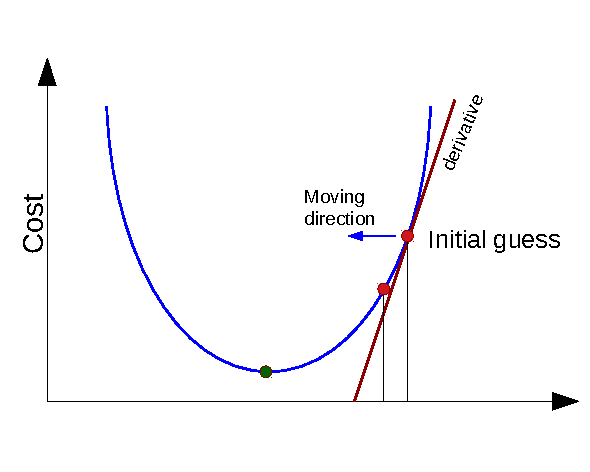
\includegraphics[width=0.5\textwidth]{images/gd1.pdf}
% \end{center}

% \end{frame}


% %%%%%%%%%%%%%%%%%%%%%%%%%%%%%%%%%%%%%%%%%%%%
% %%%%%%%%%%%%%%%%%%%%%%%%%%%%%%%%%%%%%%%%%%%%

% \begin{frame}[fragile,t]{What is a Gradient?}

% \blueb{Gradient} is the multi-dimensional analog to a \blueb{derivative}

% \begin{itemize}
%     \item $\nabla L(\theta)$ is a vector-valued function
%     \item It is a vector whose \blueb{$i$th} entry is \blueb{$i$th} partial derivative evaluated at
%     \blueb{$\theta_i$}
% \end{itemize}

% \centering

% \large
% \blueb{
% $\nabla L(\theta) =
% \begin{bmatrix}
% 	\frac{\partial L(\theta)}{\partial \theta_0}  \\
% 	\frac{\partial L(\theta)}{\partial \theta_1} \\
%    	. \\
%    	. \\
%    	. \\
%    	\frac{\partial L(\theta)}{\partial \theta_d} \\
% \end{bmatrix}
% $
%   }

% \vspace{0.5cm}

% \begin{itemize}
%     \item \textbf{Negative of gradient indicates direction of steepest descent}
%     \item We use the gradient to find out the direction of steepest descent in multidimensional space.
% \end{itemize}


% \end{frame}



% %%%%%%%%%%%%%%%%%%%%%%%%%%%%%%%%%%%%%%%%%%%%
% %%%%%%%%%%%%%%%%%%%%%%%%%%%%%%%%%%%%%%%%%%%%

% \begin{frame}[fragile, t]{Gradient Descent - Basic algorithm}

% \begin{center}
% \begin{minipage}{.55\linewidth} % find the minimal value to enclose the code

% \begin{algorithmic}

% \State $\theta^{(iter)} \gets \text{an initial guess for } \theta^*$
% \State $iter \gets 1 $
% \Repeat
%     \State $\theta^{(iter + 1 )} \gets \theta^{(iter)} - \lambda \nabla
%     L(\theta^{(iter)})$
%     \State $iter \gets iter+1$
% \Until{$(\text{Stop Condition})$ }

% \end{algorithmic}

% \end{minipage}
% \end{center}


% \vspace{0.5cm}

% \begin{itemize}
%     \item \textcolor{blue}{Here $\lambda$ is the \redb{"learning rate"}} and controls speed of convergence

%     \item \textcolor{blue}{$\nabla L(\theta_{iter})$ is the \redb{gradient} of L evaluated at iteration "$iter$" with parameter of $\theta_{iter}$ }

% 	\item Stop conditions can be different
% \end{itemize}


% \end{frame}




% %%%%%%%%%%%%%%%%%%%%%%%%%%%%%%%%%%%%%%%%%%%%
% %%%%%%%%%%%%%%%%%%%%%%%%%%%%%%%%%%%%%%%%%%%%

% \begin{frame}[fragile]{When to Stop?}
% \vspace{-.5cm}


% \begin{center}
% \begin{minipage}{.55\linewidth} % find the minimal value to enclose the code

% \begin{algorithmic}
% \State $\theta^{(iter)} \gets \text{an initial guess for } \theta^*$
% \State $iter \gets 1 $
% \Repeat
%     \State $\theta^{(iter +1 )} \gets \theta^{(iter)} - \lambda \nabla
%     L(\theta^{(iter)})$

%     \State $iter \gets iter+1$
% \Until{$(\text{Stop Condition})$ }
% \end{algorithmic}

% \end{minipage}

% \noindent\rule{6cm}{0.4pt}

% \end{center}

% % \noindent\makebox[\linewidth]{\rule{\paperwidth}{0.4pt}}



% Stop condition can be different, for example:

% \begin{itemize}
% 	\item \blueb{Maximum number of iteration is reached}    $(iter < MaxIteration)$
%     \item \blueb{Gradient $\nabla L(\theta^{(iter)}) $ or parameters are not
%     changing }$  (||\theta^{(iter+1)} - \theta^{(iter)}|| < precisionValue ) $
%     \item\blueb{Cost is not decreasing}  $ (||L(\theta^{(iter+1)}) -
%     L(\theta^{(iter)} ) || < precisionValue ) $
%     \item \blueb{Combination of the above}
% \end{itemize}

% Mostly we stop it based on number of iterations\\
%  \textit{(Early stop to avoid  "Over-fitting")}.
% \end{frame}



% %%%%%%%%%%%%%%%%%%%%%%%%%%%%%%%%%%%%%%%%%%%%
% %%%%%%%%%%%%%%%%%%%%%%%%%%%%%%%%%%%%%%%%%%%%

% % \begin{frame}[fragile, t]{Example}
% %
% % Returning to linear regression . . .
% %
% % \begin{itemize}
% %     \item \textcolor{blue}{Want a line to fit points $\langle 118, 122, 145,
% %     149, 186 \rangle$ }
% %     \item \textcolor{blue}{At time ticks $t$ in $\langle1, 2, 3, 4, 5\rangle$}
% %     \item \textcolor{blue}{Prediction $f(t|c,m) = c+m \times t$}
% %     \item \textcolor{blue}{Loss function $L(c,m) = \sum_i(f(t_i |c,m ) -x_i)^2$}
% % \end{itemize}
% %
% %
% % \end{frame}

% %%%%%%%%%%%%%%%%%%%%%%%%%%%%%%%%%%%%%%%%%%%%
% %%%%%%%%%%%%%%%%%%%%%%%%%%%%%%%%%%%%%%%%%%%%
% %
% % \begin{frame}[t]{Example}
% % Returning to linear regression . . .
% %
% % \begin{itemize}
% %     \item \textcolor{blue}{Prediction $f(t|c,m) = c+m \times t$}
% %     \item \textcolor{blue}{Loss function is Mean Squared Error $L(c,m) =  \frac{1}{N} \sum_i(f(t_i |c,m ) -x_i)^2$}
% %
% % \end{itemize}
% %
% % First we deal with c and m:
% %
% % \begin{align*}
% %     {\partial F } \over  {\partial c}  &= \Large \sum_i 2 (f(t_i |c, m ) - x_i) \\
% %     {\partial F } \over  {\partial m}  &= \Large \sum_i 2 t_i (f(t_i |c, m ) - x_i) \\
% %     So\ that \\
% %     \nabla L(c,m)  &=\langle \Large  \sum_i 2 (f(t_i |c, m ) - x_i)  , \Large \sum_i 2 t_i (f(t_i |c, m ) - x_i) \rangle\\
% % \end{align*}
% %
% % We can divide the loss by 2 to make derivative calculations simpler.
% %
% % \end{frame}

% % %%%%%%%%%%%%%%%%%%%%%%%%%%%%%%%%%%%%%%%%%%%%
% % %%%%%%%%%%%%%%%%%%%%%%%%%%%%%%%%%%%%%%%%%%%%
% %
% % \begin{frame}[t]{Grad Descent and Big Data}
% %
% % Gradient of the following form is very common
% %
% % \large{
% % \begin{align*}
% %     \nabla L(c,m)  &=\langle \Large  \sum_i 2 (f(t_i |c, m ) - x_i)  , \Large \sum_i 2 t_i (f(t_i |c, m ) - x_i) \rangle\\
% % \end{align*}
% % }
% %
% % \Large{
% % Why is this so good for "Big Data"? MapReduce?}
% %
% %
% %
% % \end{frame}


% %%%%%%%%%%%%%%%%%%%%%%%%%%%%%%%%%%%%%%%%%%%%
% %%%%%%%%%%%%%%%%%%%%%%%%%%%%%%%%%%%%%%%%%%%%

% \begin{frame}[fragile, t]{Example - Back to Multiple Linear Regression Model}
% \vspace{-.2cm}
% \begin{align*}
% y = \theta_0+ \theta_1 x_1 +  \dots + \theta_d x_d \\
% MSE=L(\Theta) =  \frac{1}{2N} \sum_{i=1}^{n} (y^{i} - (\theta_0+ \theta_1 x_1 + ... + \theta_d
% x_d))^2
% \end{align*}

% \redb{How to compute the gradient with many dimensions? }
% \pause

% Compute partial derivatives
% \large
% \blueb{
% \begin{align*}
% \frac{\partial L }{\partial  \theta_1} & =  \frac{-1}{N} \sum_{i=1}^{n} x^{(i)}_1 (y^{(i)} - (\theta_0 + \theta_1 x^{(i)}_1+ \dots  + \theta_d x^{(i)}_d)) \\
% \frac{\partial L}{\partial  \theta_2} & =  \frac{-1}{N} \sum_{i=1}^{n} x^{(i)}_2 (y^{(i)} - (\theta_0 + \theta_1 x^{(i)}_1+ \dots  + \theta_d x^{(i)}_d)) \\
% \dots  & \\
% \end{align*}
% }
% \normalsize
% Compute components of the gradients \textbf{(map operation)} and then sum them up and update weights in the next iteration \textbf{(reduce operation)}

% \end{frame}


% %%%%%%%%%%%%%%%%%%%%%%%%%%%%%%%%%%%%%%%%%%%%
% %%%%%%%%%%%%%%%%%%%%%%%%%%%%%%%%%%%%%%%%%%%%


% \begin{frame}[fragile, t]{Map Reduce Implementation}

% \begin{lstlisting}
% // initialize parameters
% iter= 0
% learningRate= 0.01
% numIteration= 400
% theta = np.zeros(noParameters)

% while (iter < maxNumIteration):
%   reduceData = myData.map(
%           // Calculate the gradients
%       )
%       .reduce(
%           // update model parameters
%           // lambda theta :  - learningRate * theta
%       )
%   iter = iter+1

% \end{lstlisting}

% In Spark you can  \blueb{reduceByKey() }or better \blueb{aggregateByKey()}


% \end{frame}




% %%%%%%%%%%%%%%%%%%%%%%%%%%%%%%%%%%%%%%%%%%%%
% %%%%%%%%%%%%%%%%%%%%%%%%%%%%%%%%%%%%%%%%%%%%

% \section{Learning Rate is Super Important}

% %%%%%%%%%%%%%%%%%%%%%%%%%%%%%%%%%%%%%%%%%%%%
% %%%%%%%%%%%%%%%%%%%%%%%%%%%%%%%%%%%%%%%%%%%%
% \begin{frame}[fragile,t]{Gradient Descent - learning rate too Small (Slow convergence)}
% The learning rate is Super important.

% \textcolor{blue}{Too small: many, many passes through the data to converge}

% \begin{center}
%     	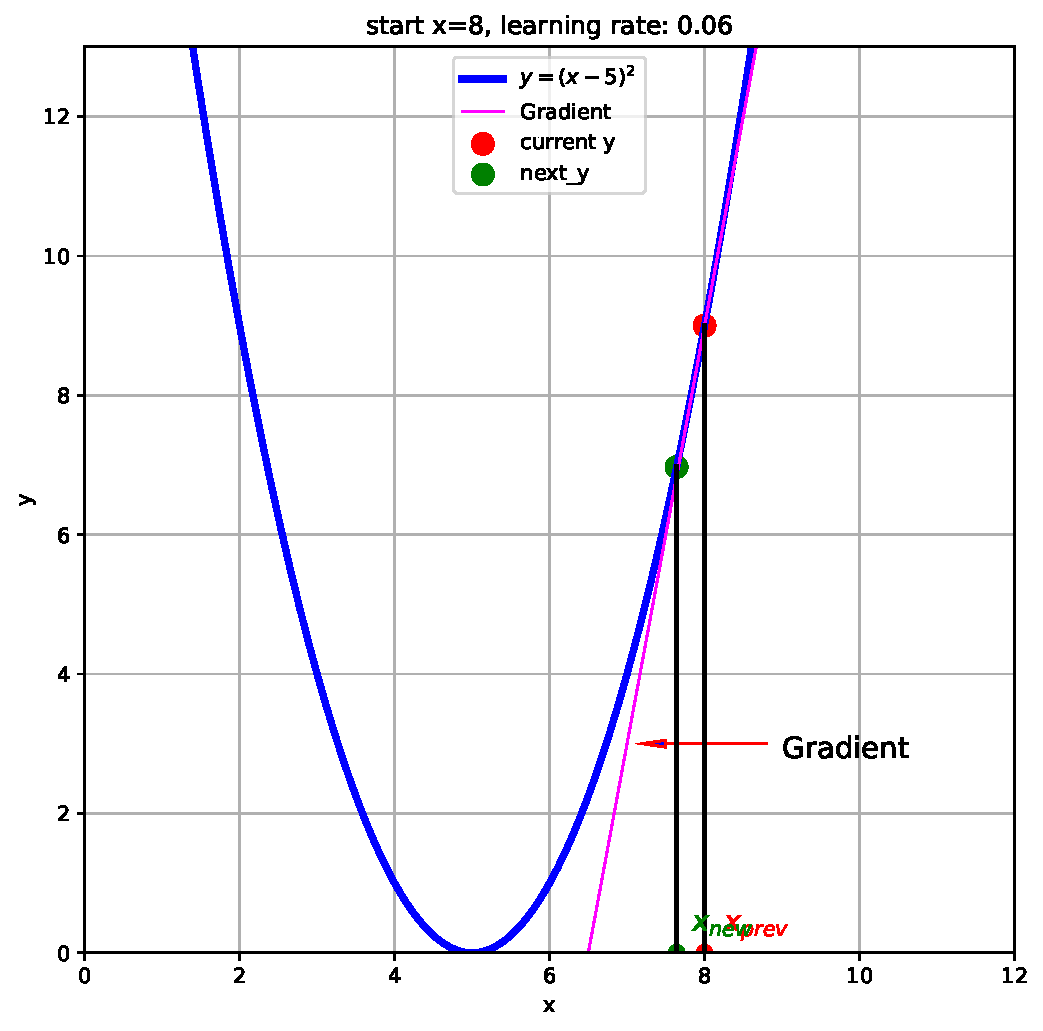
\includegraphics[width=0.5\textwidth]{images/slow.pdf}
% \end{center}



% \end{frame}


% %%%%%%%%%%%%%%%%%%%%%%%%%%%%%%%%%%%%%%%%%%%%
% %%%%%%%%%%%%%%%%%%%%%%%%%%%%%%%%%%%%%%%%%%%%
% \begin{frame}[fragile,t]{Gradient Descent}

%    \textcolor{blue}{Too large: Jumping around}

% \begin{center}
%     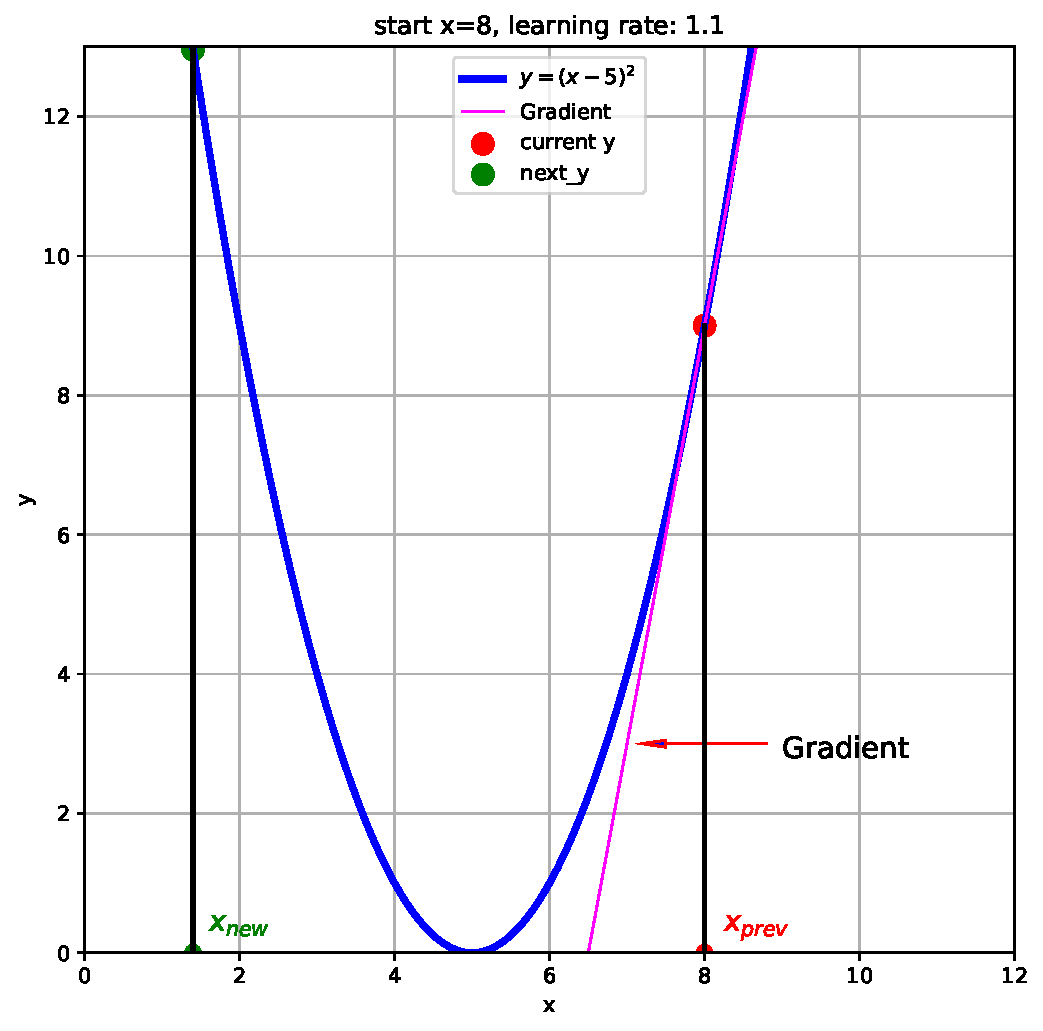
\includegraphics[width=0.5\textwidth]{images/fast.pdf}
% \end{center}

% \end{frame}




% %%%%%%%%%%%%%%%%%%%%%%%%%%%%%%%%%%%%%%%%%%%%
% %%%%%%%%%%%%%%%%%%%%%%%%%%%%%%%%%%%%%%%%%%%%
% \begin{frame}[fragile,t]{Gradient Descent - Oscillations}

%    \textcolor{blue}{Too large: oscillate into oblivion}

% \begin{center}
%     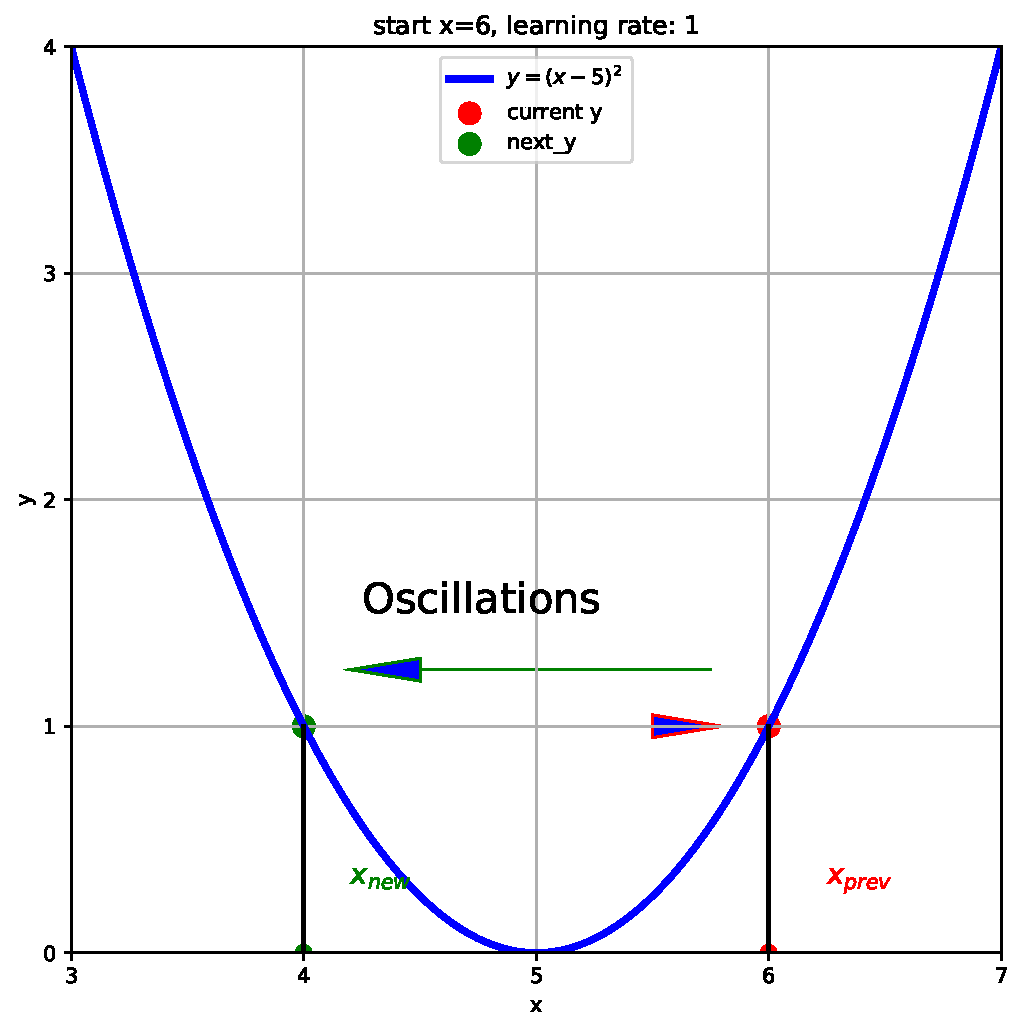
\includegraphics[width=0.6\textwidth]{images/oscillations.pdf}
% \end{center}

% \end{frame}

% %%%%%%%%%%%%%%%%%%%%%%%%%%%%%%%%%%%%%%%%%%%%
% %%%%%%%%%%%%%%%%%%%%%%%%%%%%%%%%%%%%%%%%%%%%

% \begin{frame}{Choose Learning Rate - Line Search }

% Best option (in terms of results) but \redb{most expensive}:

% \begin{itemize}
%     \item Solve another mini-optimization problem
%     \item Select $\lambda$ so as to minimize $L(\theta^{(iter)})$
%     \item It's a 1-dimensional optimization problem!
%     \item Called a line search
% \end{itemize}

% \end{frame}


% %%%%%%%%%%%%%%%%%%%%%%%%%%%%%%%%%%%%%%%%%%%%
% %%%%%%%%%%%%%%%%%%%%%%%%%%%%%%%%%%%%%%%%%%%%

% \begin{frame}[fragile, t]{Line Search}

% \begin{algorithmic}
% \State $l \gets 0$
% \State $h \gets 999999 $

% \While{$  ( h - l >\epsilon )$ }
%     \State $ h' \gets l + {{{1} \over {c}}(h-l)} $
%     \State $ l' \gets h - {{{1} \over {c}}(h-l)} $

%     \State $goodness_h \gets L(\theta^{(i)} - h' \nabla L(\theta^{(iter)}))$
%     \State $goodness_l \gets L(\theta^{(i)} - l' \nabla L(\theta^{(iter)}))$

%     \If{ $( goodness_h <  goodness_l)$}
%         \State $l \gets l'$
%     \Else
%         \State $h \gets h'$
%     \EndIf


% \EndWhile

% \end{algorithmic}
% \large


% \textcolor{red}{"Golden Section Search"} $ c = {{{1} \over {2}} (1 + \sqrt{5})} = 1.618 $


% \end{frame}



% %%%%%%%%%%%%%%%%%%%%%%%%%%%%%%%%%%%%%%%%%%%%
% %%%%%%%%%%%%%%%%%%%%%%%%%%%%%%%%%%%%%%%%%%%%

% \begin{frame}[fragile, t]{Other Ways To Choose Learning Rate - "Bold Driver"}

% Line search is very costly!

% One other standard method is \textcolor{red}{"Bold Driver"}

% \begin{itemize}
%     \item \textcolor{blue}{Make a very conservative initial guess for $\lambda$  } \\
%    \textcolor{blue}{At each iteration, compute the cost $L(\Theta^{(iter)} )$ }

%     \item \textcolor{blue}{Better than last time?
%      \\
%      $ \lambda \gets   1.05 \times \lambda $}
%       \\
%      \brownb{If cost decreases, increase learning rate}
% 		\\
%     \item \textcolor{blue}{Worse than last time? \\
%     $ \lambda \gets  0.5 \times \lambda$}
%       \\
% 	\brownb{If cost increases, decrease rate}
% \end{itemize}

% \textbf{This would be then just one evaluation of loss function per iteration!}
% \end{frame}


% %%%%%%%%%%%%%%%%%%%%%%%%%%%%%%%%%%%%%%%%%%%%
% %%%%%%%%%%%%%%%%%%%%%%%%%%%%%%%%%%%%%%%%%%%%

% \begin{frame}{Cost Monitoring - "Bold Driver" vs. Constant Learning Rates}

% \normalsize
% \begin{center}
%     	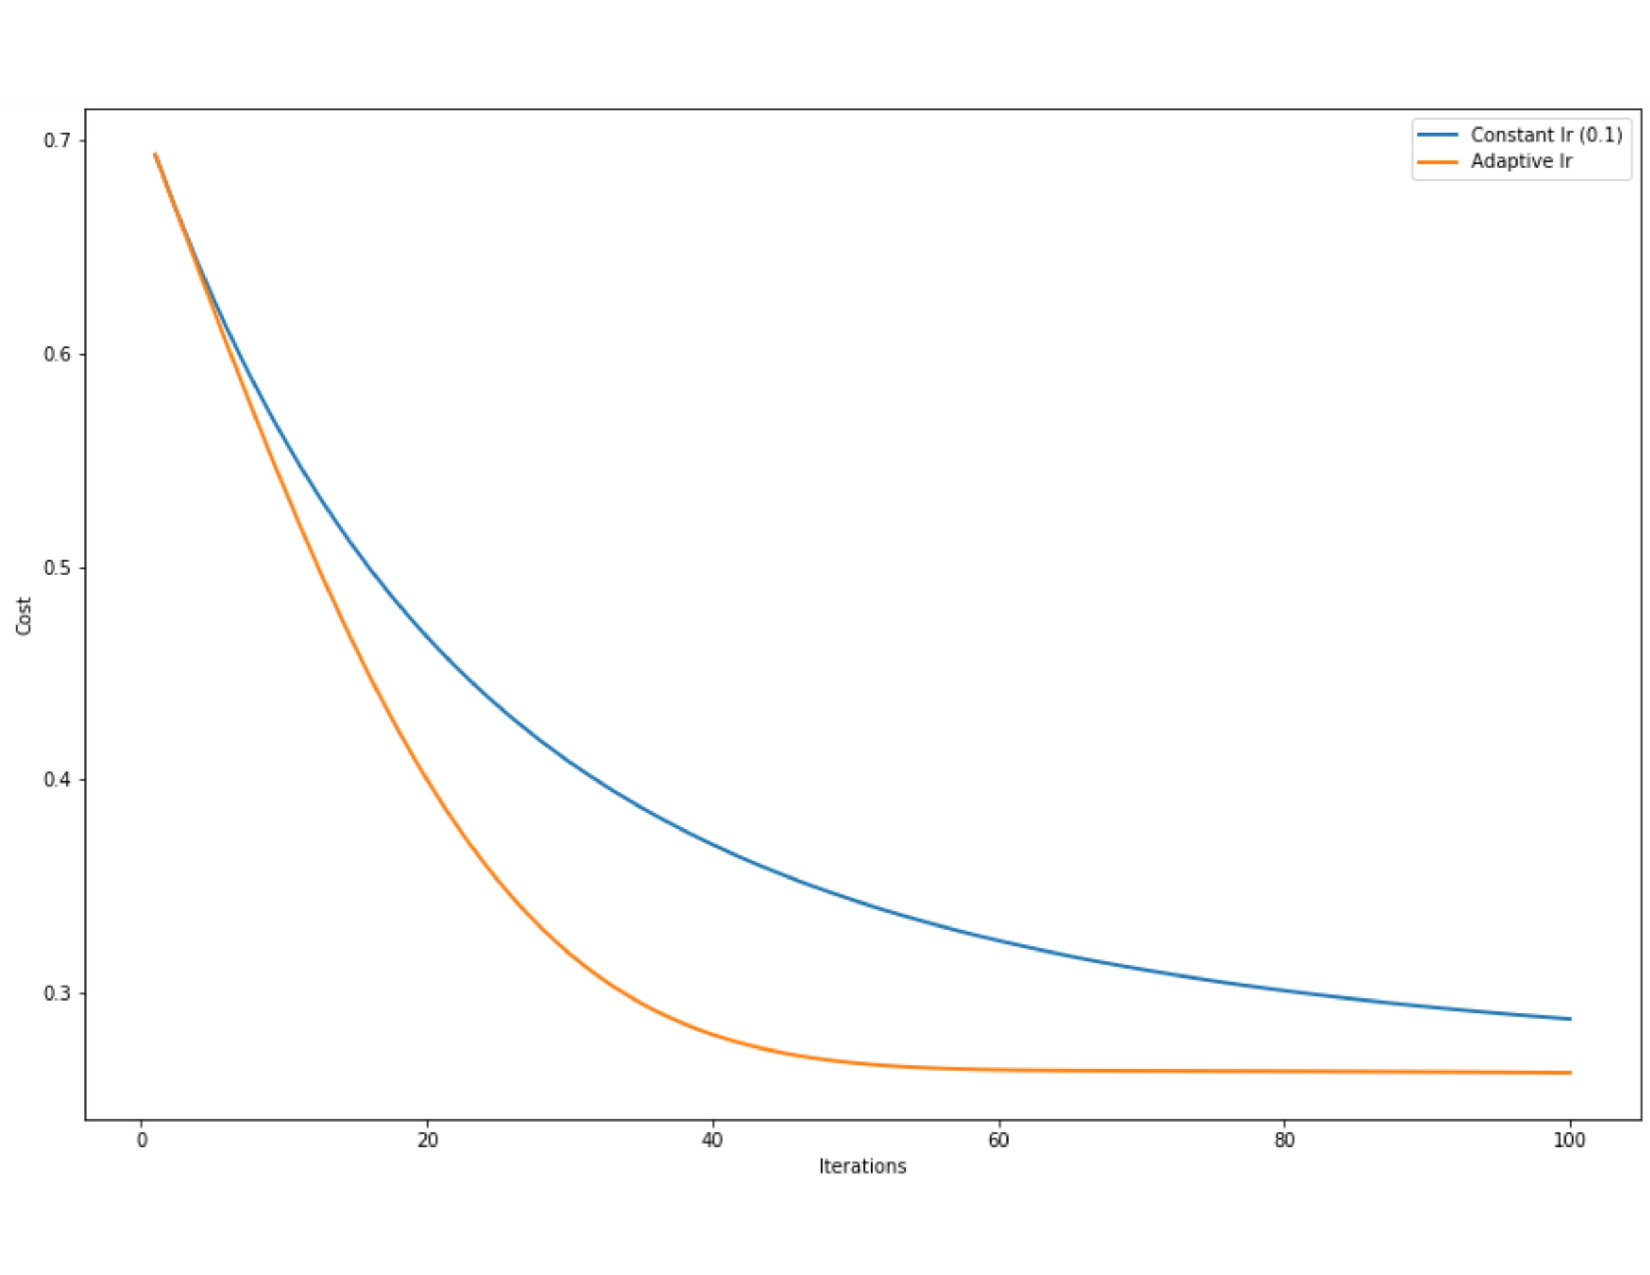
\includegraphics[width=0.75\textwidth]{images/graph02.pdf}
% \end{center}

% \vspace{-.7cm}

% Text Classification with Logistic regression (20k Dimensions Term Frequencies) .


% \begin{itemize}
%   \item Horizontal axis is number of iterations
%   \item Vertical axis shows value of negative log-likelihood
% \end{itemize}

% \end{frame}

% %%%%%%%%%%%%%%%%%%%%%%%%%%%%%%%%%%%%%%%%%%%%
% %%%%%%%%%%%%%%%%%%%%%%%%%%%%%%%%%%%%%%%%%%%%

% \begin{frame}{Text Classification with Logistic regression - Different Learning Rate}

% \vspace{-.4cm}
% \begin{center}
%     	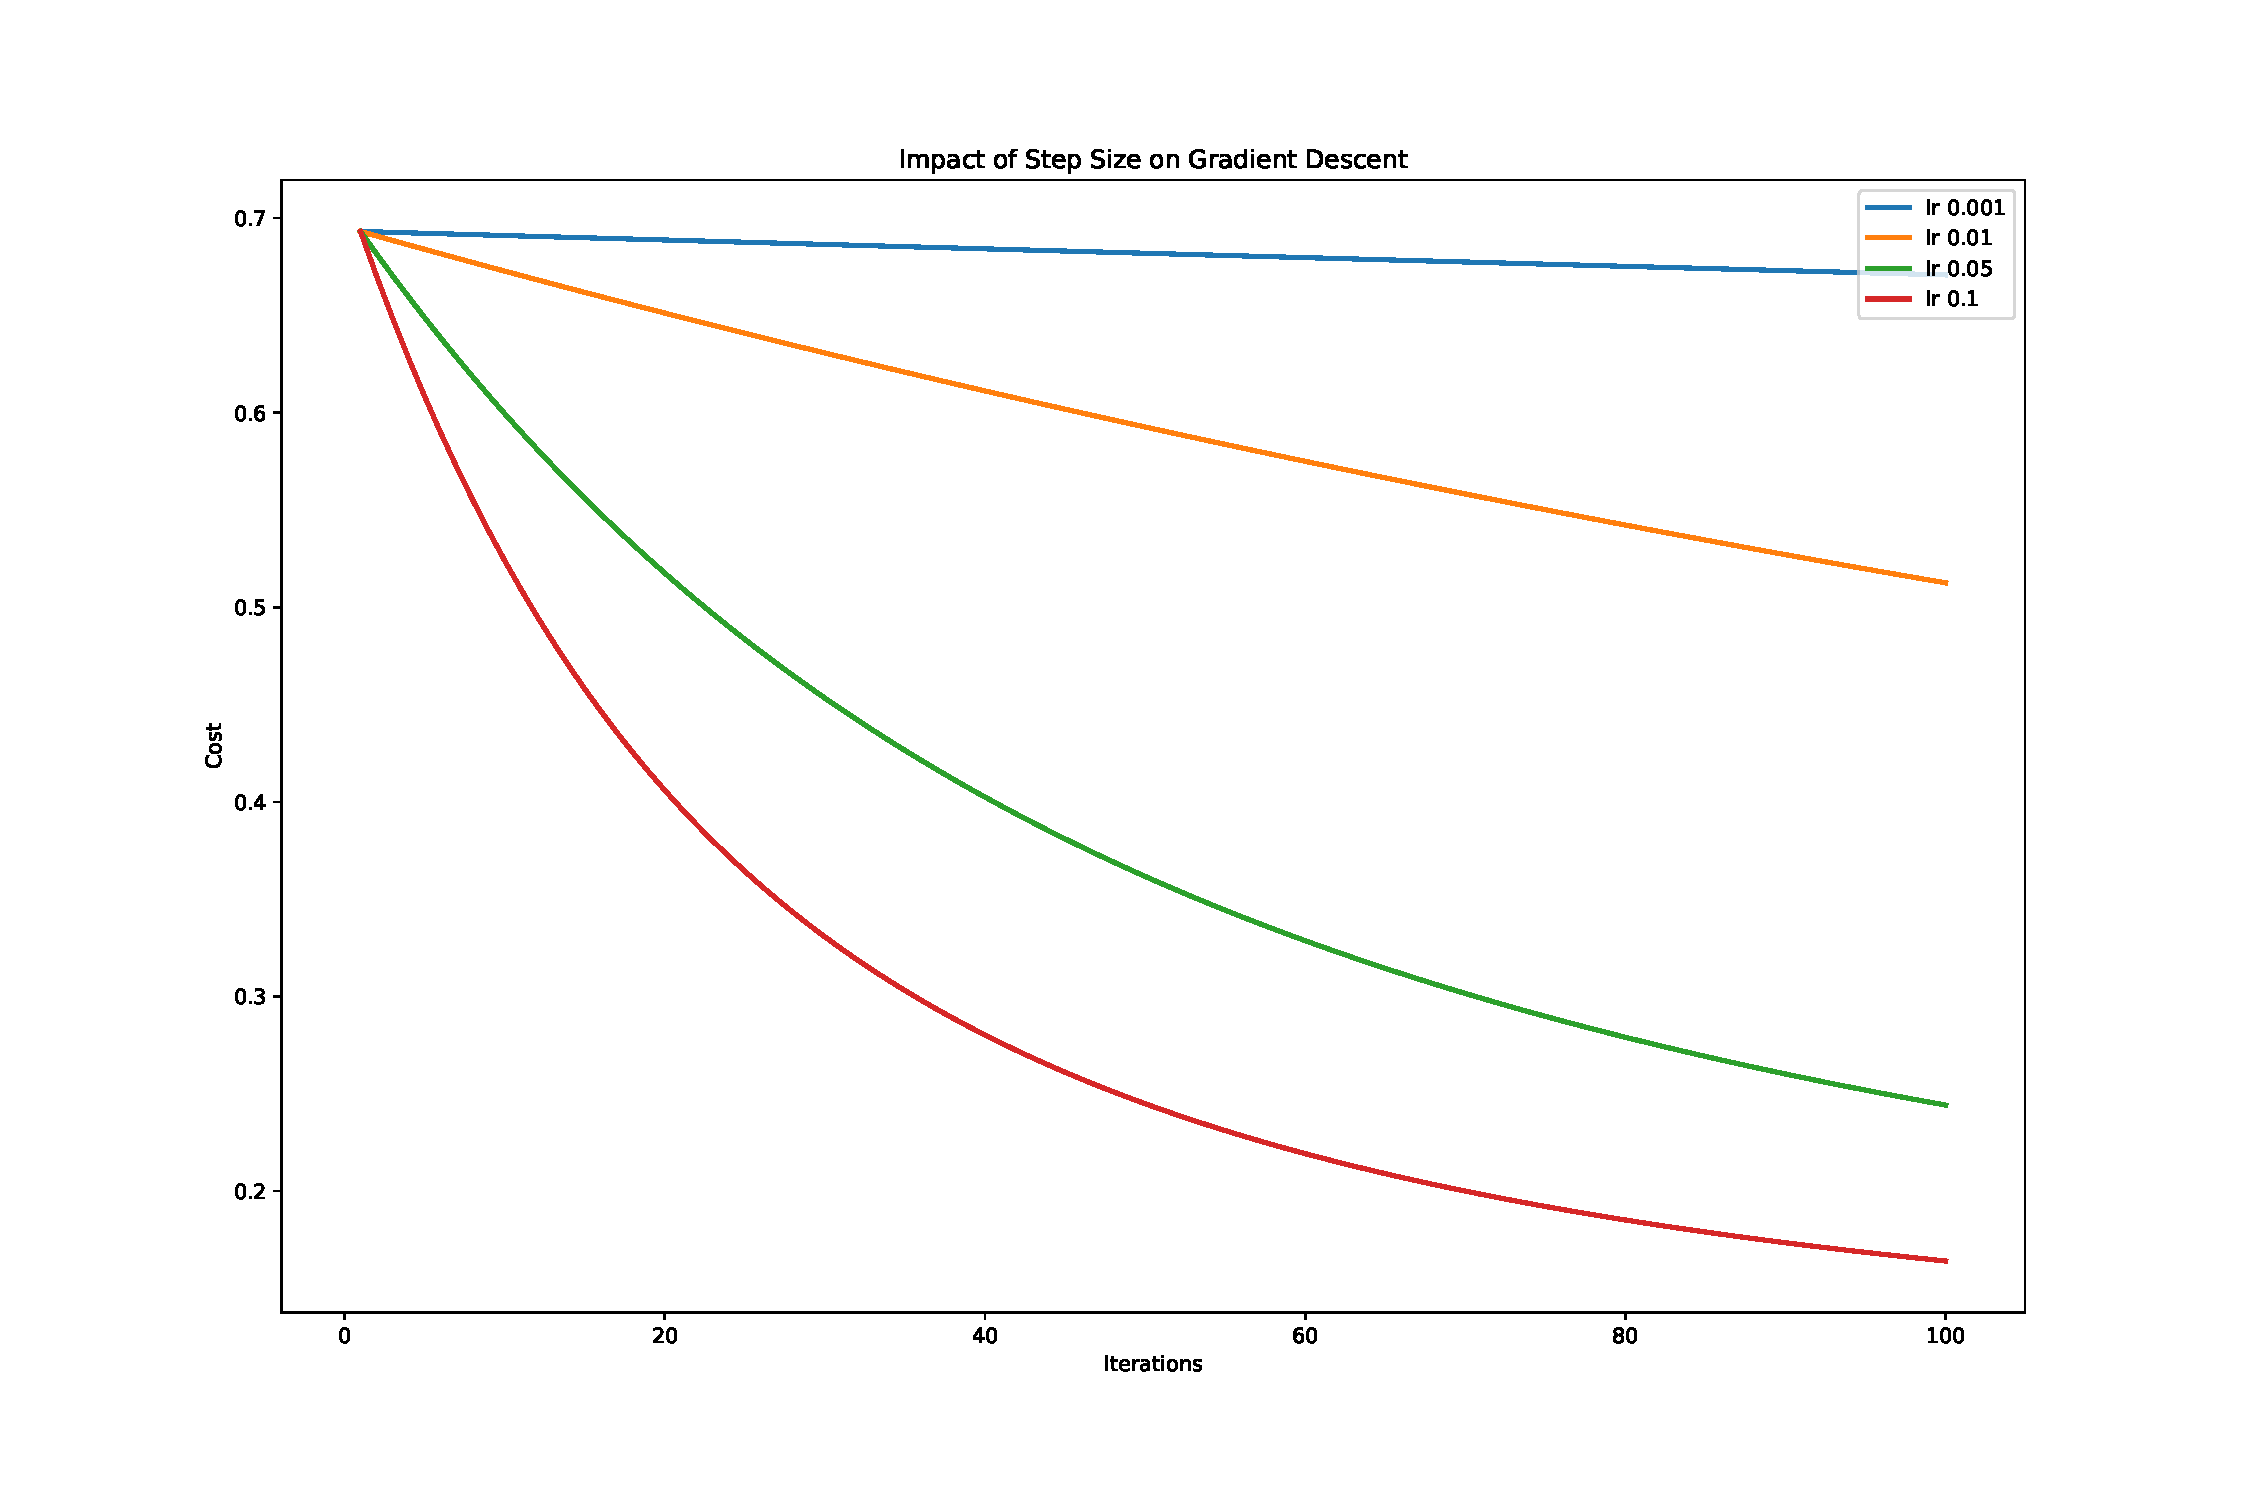
\includegraphics[width=0.9\textwidth]{images/DifferentLearningRate.pdf}
% \end{center}

% \vspace{-.5cm}

% The same Text Classification with 20k Dimensions,  term frequencies of words

% \end{frame}





% %%%%%%%%%%%%%%%%%%%%%%%%%%%%%%%%%%%%%%%%%%%%
% %%%%%%%%%%%%%%%%%%%%%%%%%%%%%%%%%%%%%%%%%%%%

% \begin{frame}{Example  - Very Large Learning Rate}

% \vspace{-.4cm}
% \begin{center}
%     	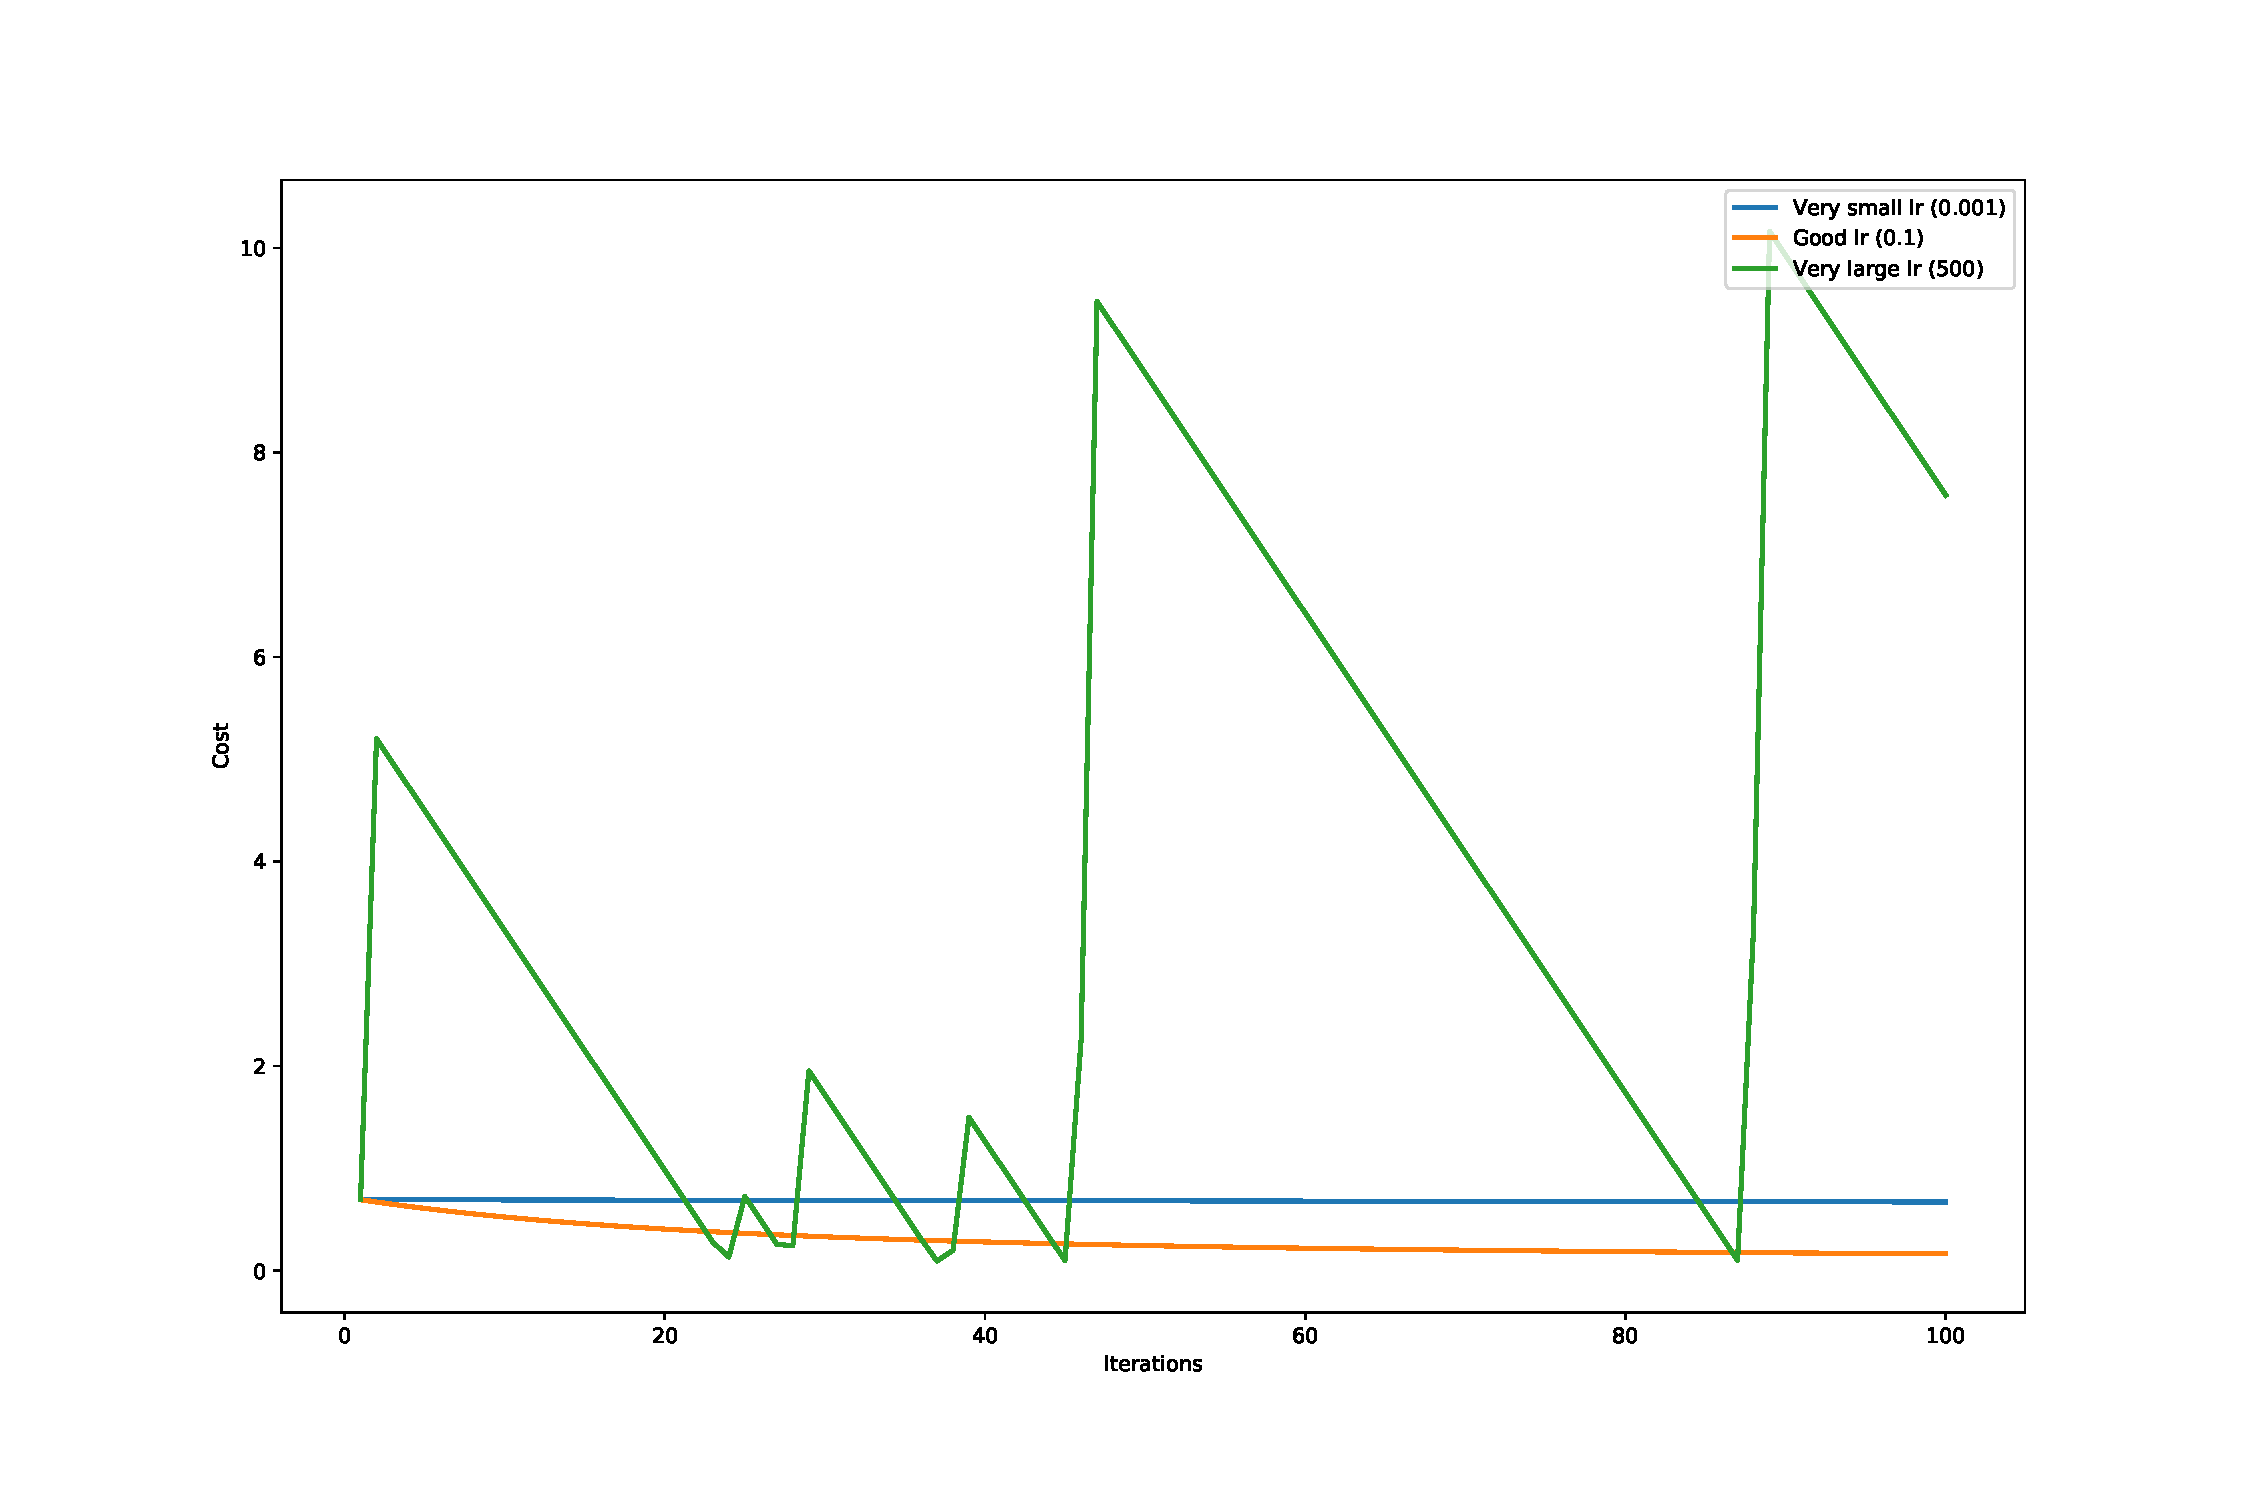
\includegraphics[width=0.7\textwidth]{images/VeryLargeAndSmallLearningRate.pdf}
% \end{center}

% \vspace{-.5cm}

% The same Text classification with 20k Dimensions,  term frequencies of words


% \begin{itemize}
% 	\item Very small learning rate of 0.001
% 	\item Very Large learning rate
% 	\item Good working learning rate.
% \end{itemize}

% \end{frame}




% %%%%%%%%%%%%%%%%%%%%%%%%%%%%%%%%%%%%%%%%%%%%
% %%%%%%%%%%%%%%%%%%%%%%%%%%%%%%%%%%%%%%%%%%%%

% \begin{frame}{Text Classification with Logistic regression - Large Learning Rate}

% \vspace{-.4cm}
% \begin{center}
%     	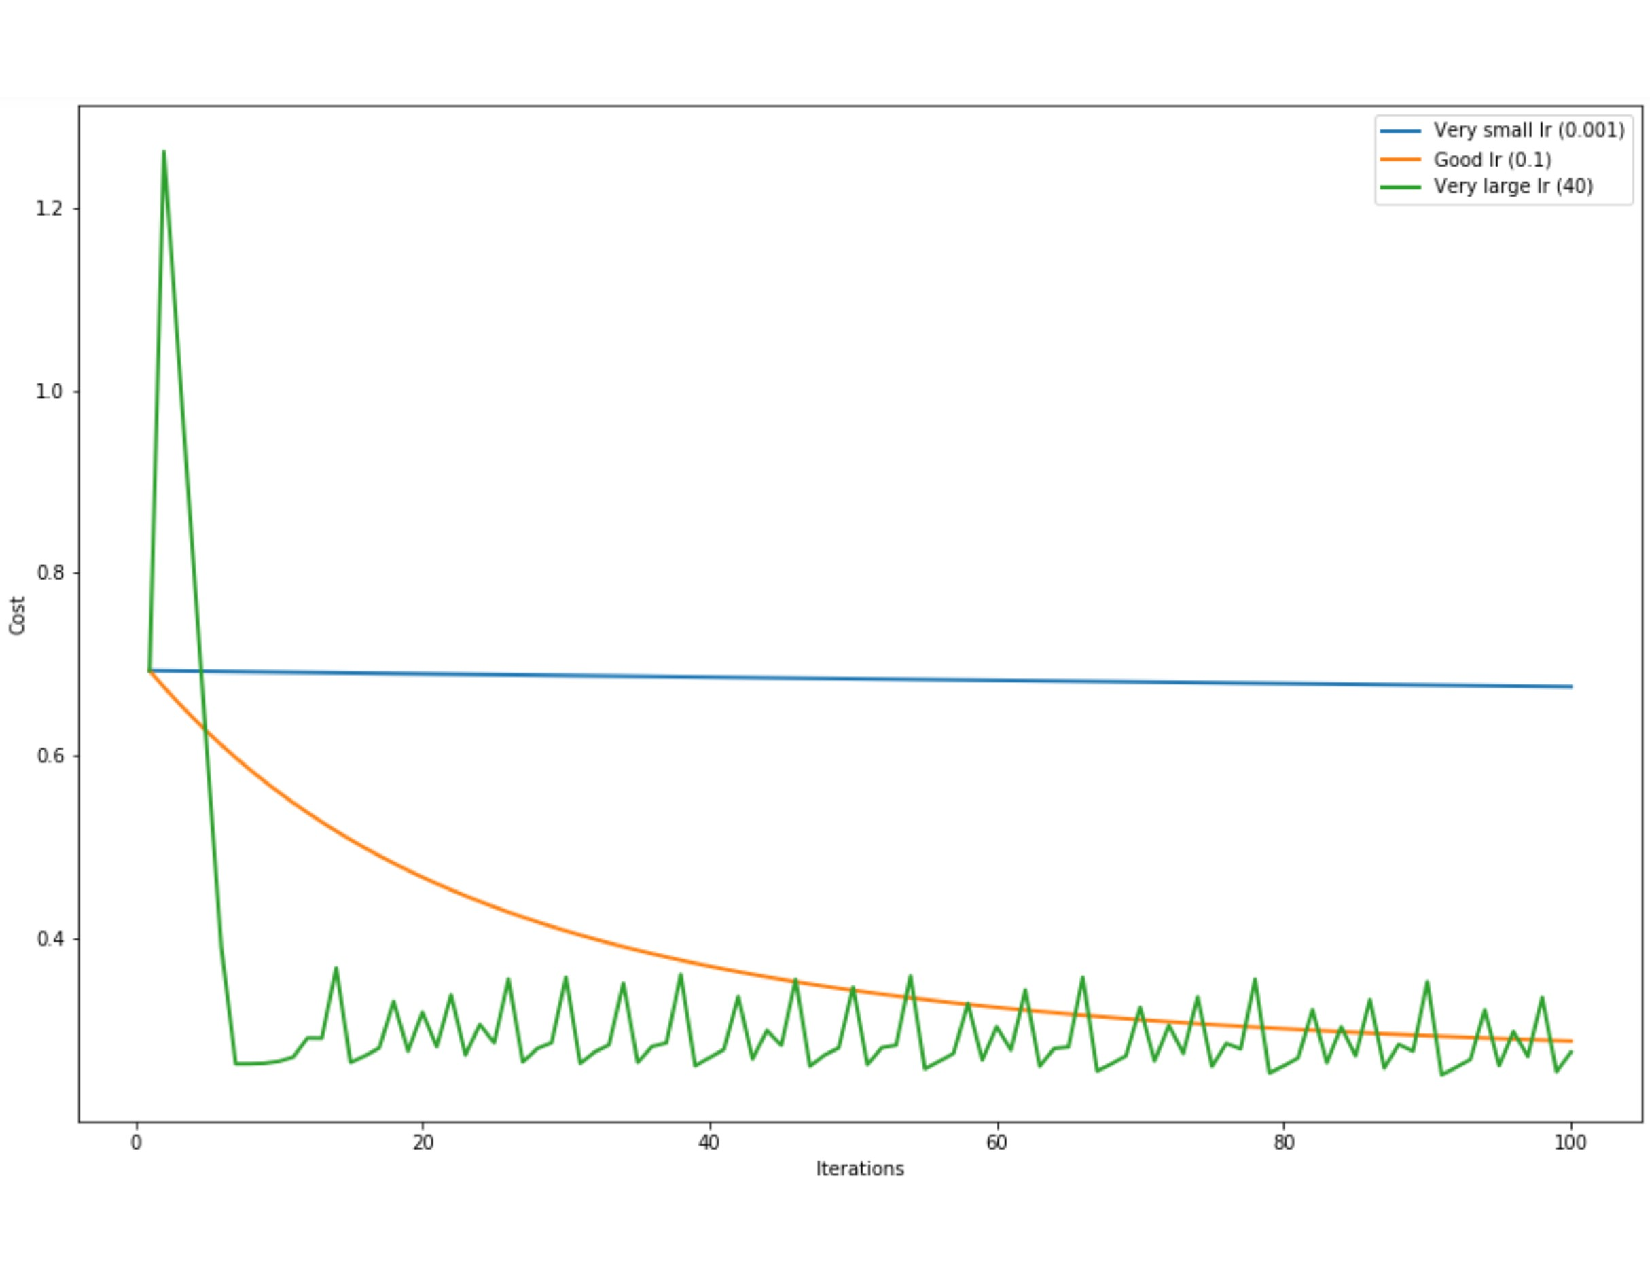
\includegraphics[width=0.7\textwidth]{images/graph01.pdf}
% \end{center}

% \vspace{-.5cm}

% 20k Dimensions,  term frequencies of words

% \begin{itemize}
% 	\item Very small learning rate of 0.001
% 	\item Large learning rate
% 	\item Good working learning rate.
% \end{itemize}

% \end{frame}




% %%%%%%%%%%%%%%%%%%%%%%%%%%%%%%%%%%%%%%%%%%%%
% %%%%%%%%%%%%%%%%%%%%%%%%%%%%%%%%%%%%%%%%%%%%
% \section{Variations of Gradient Descent}

% \begin{frame}{Variations of Gradient Descent}

% Depending on Size of data that we use in each iteration:

% \begin{itemize}
%     \item \brownb{Full Batch Gradient Descent} (Using the whole data set (size n))
%     \item \brownb{Stochastic Gradient Descent (SGD)}  (Using one sample per iteration (size 1))
%     \item \blueb{Mini Batch Gradient Descent} (Using a mini batch of data (size $m < n$))
% \end{itemize}

% Some times people refer to SGD  as  mini batch.
% \end{frame}


% %%%%%%%%%%%%%%%%%%%%%%%%%%%%%%%%%%%%%%%%%%%%
% %%%%%%%%%%%%%%%%%%%%%%%%%%%%%%%%%%%%%%%%%%%%

% \begin{frame}{Stochastic Gradient Descent}
% Calculate the gradient of a single sample and update parameters in
%     each iterations

% \begin{itemize}
%     \item Pick up samples for update by \textbf{sequential read (pass over the data} - do not
%     take random sample from a big data set in each iterations  - computationally expensive)


%      \item It is noisy and sometimes  will do lots of iterations
%     \item Do not be afraid of \textbf{non-convex functions}, SGD can help to \blueb{get out of local minimums}.

%     \item It is a widely applied approach

%     \item SGD is often faster in producing good results.

% \end{itemize}
% \end{frame}



% %%%%%%%%%%%%%%%%%%%%%%%%%%%%%%%%%%%%%%%%%%%%
% %%%%%%%%%%%%%%%%%%%%%%%%%%%%%%%%%%%%%%%%%%%%

% \begin{frame}{Mini-Batch Gradient Descent}

% Something between Stochastic and Full-batch

% \begin{itemize}
%     \item Pick up mini batch samples for update by sequential pass over the data and use it to update
%     \item Batch gradient descent has  better convergence rates than stochastic
%     gradient descent in theory.
%     \item But we may not to pursue to converge fast (presumably results in overfitting)

%     \item Depending on size, can help to  out of local minimums.
% \end{itemize}


% Implementation Tips:
% \begin{itemize}
%     \item Use mini-batch data size of 64, 256, 512, ... (power of 2))
%     \item Make sure that mini-batch data fits in CPU/GPU memory
% \end{itemize}


% \end{frame}


% %%%%%%%%%%%%%%%%%%%%%%%%%%%%%%%%%%%%%%%%%%%%
% %%%%%%%%%%%%%%%%%%%%%%%%%%%%%%%%%%%%%%%%%%%%

% \begin{frame}{Implementation Tips:}


% \begin{itemize}
%     \item \blueb{Monitor the costs in each iteration to check if it decreases.}
%     \item \textbf{Map} to calculate gradients, \textbf{Reduce} to update the weights
%     \item Use vectorization of computations (run bulk operations, e.g., use numpy inside Spark RDDs or Spark Dataframes)
% \end{itemize}

% \end{frame}


% %%%%%%%%%%%%%%%%%%%%%%%%%%%%%%%%%%%%%%%%%%%%
% %%%%%%%%%%%%%%%%%%%%%%%%%%%%%%%%%%%%%%%%%%%%

% \begin{frame}{Issues of Gradient Descent}


% \begin{itemize}
%     \item You can find local min/max and not Global
%     \item There is no grantee that you can find the global minimum
%     \item All depends on Starting point, Step-Size and Function type.
% \end{itemize}

% The main problem is : \\
% \redb{Oscillate into oblivion}

% \end{frame}





% %%%%%%%%%%%%%%%%%%%%%%%%%%%%%%%%%%%%%%%%%%%%
% %%%%%%%%%%%%%%%%%%%%%%%%%%%%%%%%%%%%%%%%%%%%

% \begin{frame}[fragile,t]{Gradient Descent with Momentum }

% \textbf{A momentum} is a moving average of our gradients.


% \centering
% \Large
% \blueb{
% \begin{align*}
% V^{(iter)} = &  \beta   V^{iter - 1} +  (1 - \beta ) \nabla L(W, X, y) \\
% W^{(iter+1)} = & W^{(iter)} - \lambda   V^{(iter)}
% \end{align*}
% }

% \begin{itemize}
% 	\item $\beta $ is a positive number

% 	\item $\lambda $ is learning rate

% 	\item $ L(W, X, y)$ is cost function

% 	\item $W$ is vector of weights (model parameters)
% \end{itemize}

% \end{frame}







% %%%%%%%%%%%%%%%%%%%%%%%%%%%%%%%%%%%%%%%%%%%%
% %%%%%%%%%%%%%%%%%%%%%%%%%%%%%%%%%%%%%%%%%%%%

% \begin{frame}{Further methods }



% \begin{itemize}

%   	\item Adaptive gradient algorithm (AdaGrad)
%     \item Root Mean Square Propagation (RMSProp)
%     \item \brownb{Adaptive Moment Estimation (Adam)}
%     \item ...
% \end{itemize}

% \end{frame}





% %%%%%%%%%%%%%%%%%%%%%%%%%%%%%%%%%%%%%%%%%%%%
% %%%%%%%%%%%%%%%%%%%%%%%%%%%%%%%%%%%%%%%%%%%%

% \begin{frame}{ADAM: A METHOD FOR STOCHASTIC OPTIMIZATION }


% \begin{center}
%     	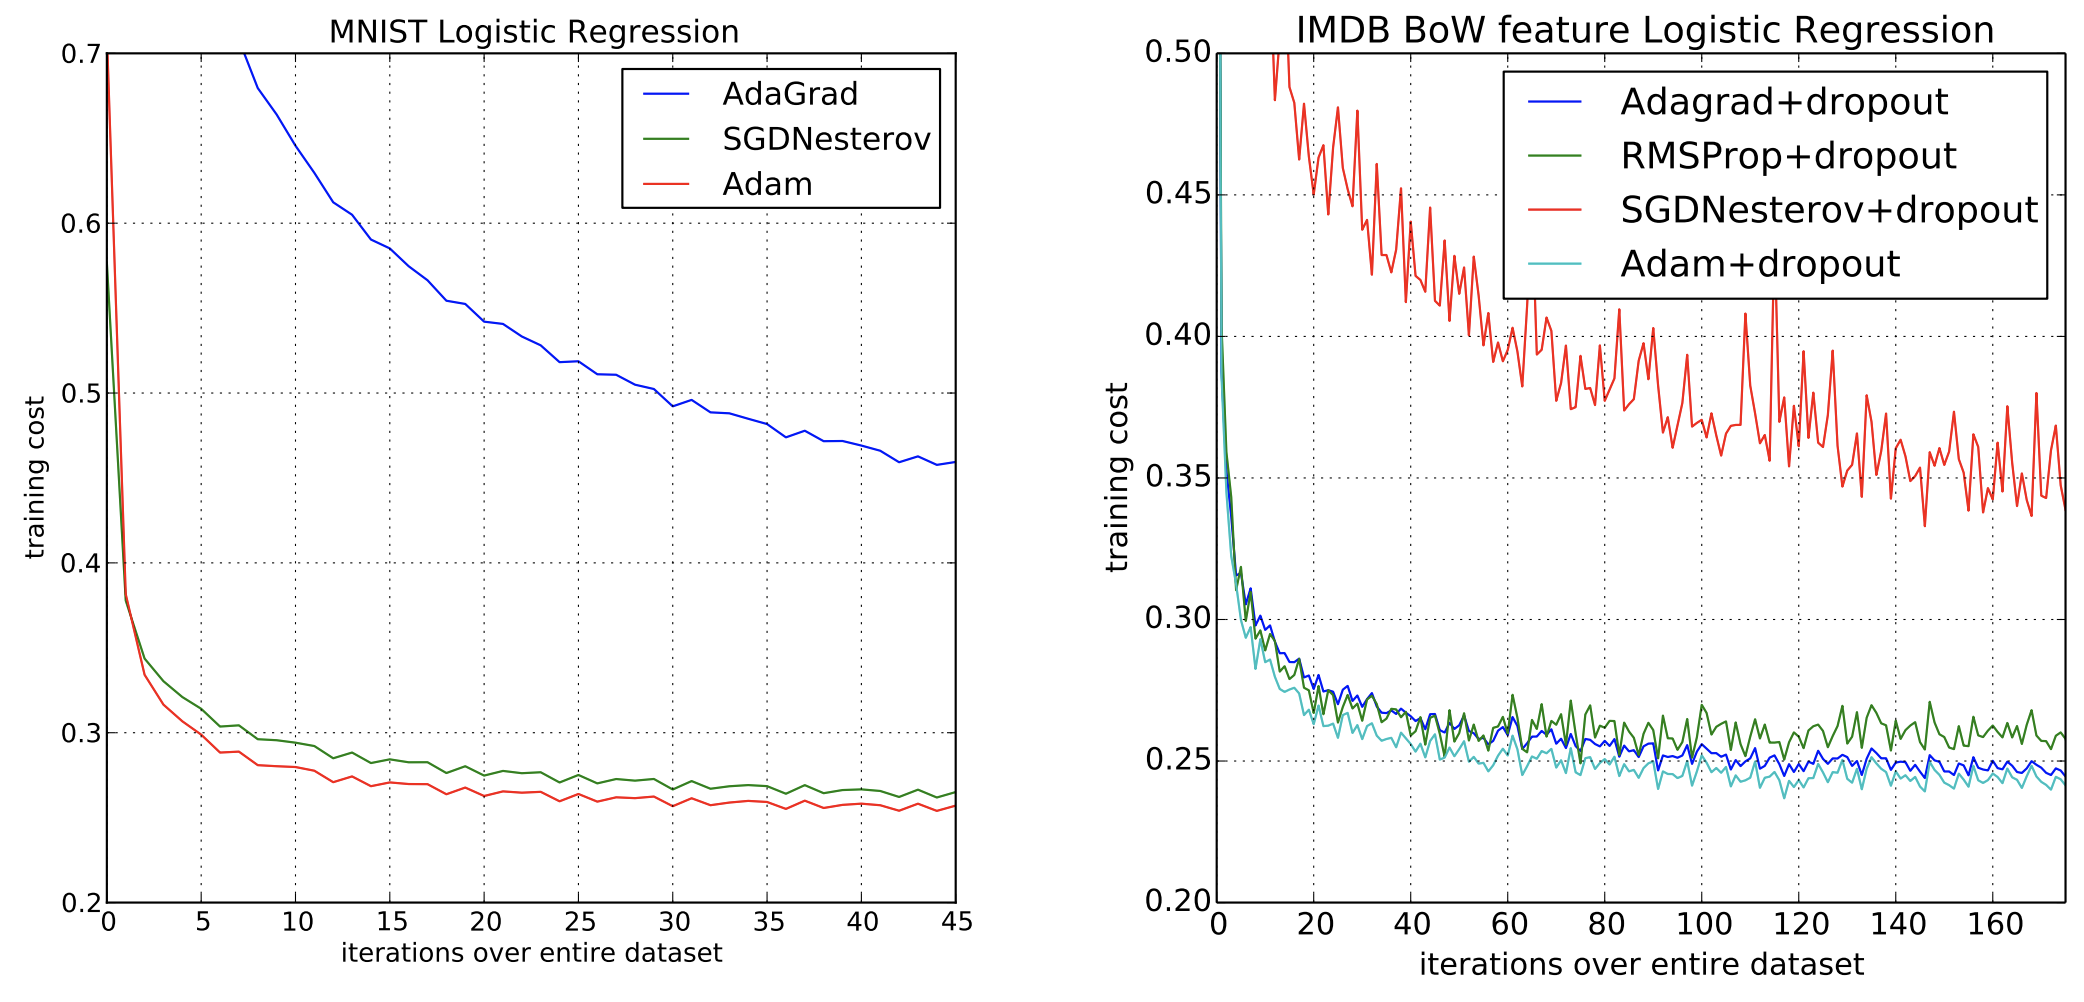
\includegraphics[width=0.9\textwidth]{images/Adam.png}
% \end{center}

% Logistic regression training negative log likelihood on MNIST images and IMDB movie
% reviews with 10,000 bag-of-words (BoW) feature vectors.

% (Image from Kingma et. al 2017)
% \end{frame}







% %%%%%%%%%%%%%%%%%%%%%%%%%%%%%%%%%%%%%%%%%%%%
% %%%%%%%%%%%%%%%%%%%%%%%%%%%%%%%%%%%%%%%%%%%%

% \begin{frame}{Summary}

% \brownb{Gradient Descent is a great optimization algorithm}

% \begin{itemize}
%     \item Gradient descent is a \textbf{first-order} iterative optimization algorithm
%     and is easy to use.
%     \item Widely applicable in many different machine learning methods
%     \item But convergence can be slow
% \end{itemize}




% \end{frame}


% %%%%%%%%%%%%%%%%%%%%%%%%%%%%%%%%%%%%%%%%%%%%
% %%%%%%%%%%%%%%%%%%%%%%%%%%%%%%%%%%%%%%%%%%%%
% %
% \begin{frame}[t]{Some of the related publications }

% \footnotesize
% \begin{itemize}
%   	\item  Diederik P. Kingma, Jimmy Ba (2015). \textit{Adam: A Method for Stochastic Optimization.} In proceeding of ICLR 2015: San Diego, CA, USA

%   	\item John Duchi, Elad Hazan, and Yoram Singer (2011). \textit{Adaptive
%   	Subgradient Methods for Online Learning and Stochastic Optimization.} Journal of Machine Learning Research, 12:2121–2159, 2011.
%   	\item Timothy Dozat (2016). \textit{Incorporating Nesterov Momentum into
%   	Adam.} ICLR  	Workshop, (1):2013–2016, 2016.

%     \item Bottou, Léon (1998). \textit{Online Algorithms and Stochastic Approximations.} Online Learning and Neural Networks. Cambridge University Press. ISBN 978-0-521-65263-6

%     \item Bottou, Léon (2010). \textit{Large-scale machine learning with SGD.} Proceedings of COMPSTAT’2010. Physica-Verlag HD, 2010. 177-186.

%     \item Bottou, Léon (2012). \textit{SGD tricks. Neural Networks: Tricks of the Trade.} Springer Berlin Heidelberg, 2012. 421-436.

% \end{itemize}

% \end{frame}



% %%%%%%%%%%%%%%%%%%%%%%%%%%%%%%%%%%%%%%%%%%%%
% %%%%%%%%%%%%%%%%%%%%%%%%%%%%%%%%%%%%%%%%%%%%
% \section{Extra Slides}


% %%%%%%%%%%%%%%%%%%%%%%%%%%%%%%%%%%%%%%%%%%%%
% %%%%%%%%%%%%%%%%%%%%%%%%%%%%%%%%%%%%%%%%%%%%
% \section{Example - Doing Regression \\ Computation can be expensive}

% \begin{frame}[fragile, t ]{Example - Doing Regression}
% We have a set of training data like \\

% \begin{itemize}
% \item Data Matrix of  \blueb{$X \in  \mathbb{R}^{n \times d}$},  with Labels \blueb{$Y \in  \mathbb{R}^{n  \times 1}$}
%     \item Linear Regression Model :
% \large
% \begin{align*}
% y = & \theta_0+ \theta_1 x_1 + \theta_2 x_2 + ... + \theta_d x_d + e \\
% \text{The same in matrix form:   } Y_{n \times 1 } = & X_{n \times d}   \Theta_{d \times 1 }  + e_{n \times 1}
% \end{align*}
%  \normalsize

%     \pause
%     \item We are looking for a vector of parameters (set of weights)

%     \blueb{$\Theta \in \mathbb{R}^{d \times 1}$} to minimize
% \begin{center}
% \large
% $MSE=L(\Theta) = \frac{1}{N} e^T e =  \frac{1}{N}  (y^T y - 2 \Theta^T X^T  y + \Theta^T X^T  X \Theta )$
%  % \frac{1}{N} \sum_{i=1}^{n} (y_i - (\theta_0+ \theta_1 x_1 + ... + \theta_d x_d))^2$
% \end{center}
% \normalsize
% \end{itemize}
% \pause

% Finding exact  solution:

% \begin{itemize}
%   \item This function is a \brownb{convex function}.
%   \item Take the derivative and set it to zero

% \Large
% \blueb{
%   $ \frac{d }{d  \Theta}  L(\Theta)= -2 X^T (Y - X \Theta)  = 0 $
% }
% \end{itemize}

%  We set the above to zero and will get
% \Large
% \begin{center}
% \blueb{$\Theta = (X^T X )^{-1} X^T Y$}
% \end{center}

% \end{frame}










\end{document}
